\documentclass[]{article}
\usepackage{lmodern}
\usepackage{amssymb,amsmath}
\usepackage{ifxetex,ifluatex}
\usepackage{fixltx2e} % provides \textsubscript
\ifnum 0\ifxetex 1\fi\ifluatex 1\fi=0 % if pdftex
  \usepackage[T1]{fontenc}
  \usepackage[utf8]{inputenc}
\else % if luatex or xelatex
  \ifxetex
    \usepackage{mathspec}
    \usepackage{xltxtra,xunicode}
  \else
    \usepackage{fontspec}
  \fi
  \defaultfontfeatures{Mapping=tex-text,Scale=MatchLowercase}
  \newcommand{\euro}{€}
    \setmainfont{Calibri}
    \setsansfont{Gill Sans Light}
    \setmonofont[Mapping=tex-ansi]{Gill Sans Light}
\fi
% use upquote if available, for straight quotes in verbatim environments
\IfFileExists{upquote.sty}{\usepackage{upquote}}{}
% use microtype if available
\IfFileExists{microtype.sty}{%
\usepackage{microtype}
\UseMicrotypeSet[protrusion]{basicmath} % disable protrusion for tt fonts
}{}
\usepackage[a4paper]{geometry}
\usepackage{color}
\usepackage{fancyvrb}
\newcommand{\VerbBar}{|}
\newcommand{\VERB}{\Verb[commandchars=\\\{\}]}
\DefineVerbatimEnvironment{Highlighting}{Verbatim}{commandchars=\\\{\}}
% Add ',fontsize=\small' for more characters per line
\usepackage{framed}
\definecolor{shadecolor}{RGB}{48,48,48}
\newenvironment{Shaded}{\begin{snugshade}}{\end{snugshade}}
\newcommand{\KeywordTok}[1]{\textcolor[rgb]{0.94,0.87,0.69}{{#1}}}
\newcommand{\DataTypeTok}[1]{\textcolor[rgb]{0.87,0.87,0.75}{{#1}}}
\newcommand{\DecValTok}[1]{\textcolor[rgb]{0.86,0.86,0.80}{{#1}}}
\newcommand{\BaseNTok}[1]{\textcolor[rgb]{0.86,0.64,0.64}{{#1}}}
\newcommand{\FloatTok}[1]{\textcolor[rgb]{0.75,0.75,0.82}{{#1}}}
\newcommand{\CharTok}[1]{\textcolor[rgb]{0.86,0.64,0.64}{{#1}}}
\newcommand{\StringTok}[1]{\textcolor[rgb]{0.80,0.58,0.58}{{#1}}}
\newcommand{\CommentTok}[1]{\textcolor[rgb]{0.50,0.62,0.50}{{#1}}}
\newcommand{\OtherTok}[1]{\textcolor[rgb]{0.94,0.94,0.56}{{#1}}}
\newcommand{\AlertTok}[1]{\textcolor[rgb]{1.00,0.81,0.69}{{#1}}}
\newcommand{\FunctionTok}[1]{\textcolor[rgb]{0.94,0.94,0.56}{{#1}}}
\newcommand{\RegionMarkerTok}[1]{\textcolor[rgb]{0.80,0.80,0.80}{{#1}}}
\newcommand{\ErrorTok}[1]{\textcolor[rgb]{0.76,0.75,0.62}{{#1}}}
\newcommand{\NormalTok}[1]{\textcolor[rgb]{0.80,0.80,0.80}{{#1}}}
\usepackage{graphicx}
\makeatletter
\def\maxwidth{\ifdim\Gin@nat@width>\linewidth\linewidth\else\Gin@nat@width\fi}
\def\maxheight{\ifdim\Gin@nat@height>\textheight\textheight\else\Gin@nat@height\fi}
\makeatother
% Scale images if necessary, so that they will not overflow the page
% margins by default, and it is still possible to overwrite the defaults
% using explicit options in \includegraphics[width, height, ...]{}
\setkeys{Gin}{width=\maxwidth,height=\maxheight,keepaspectratio}
\ifxetex
  \usepackage[setpagesize=false, % page size defined by xetex
              unicode=false, % unicode breaks when used with xetex
              xetex]{hyperref}
\else
  \usepackage[unicode=true]{hyperref}
\fi
\hypersetup{breaklinks=true,
            bookmarks=true,
            pdfauthor={ManyLabs2 (Corresponding coder: Fred Hasselman)},
            pdftitle={ManyLabs2 Data Cleaning},
            colorlinks=true,
            citecolor=blue,
            urlcolor=blue,
            linkcolor=magenta,
            pdfborder={0 0 0}}
\urlstyle{same}  % don't use monospace font for urls
\setlength{\parindent}{0pt}
\setlength{\parskip}{6pt plus 2pt minus 1pt}
\setlength{\emergencystretch}{3em}  % prevent overfull lines
\setcounter{secnumdepth}{0}

%%% Use protect on footnotes to avoid problems with footnotes in titles
\let\rmarkdownfootnote\footnote%
\def\footnote{\protect\rmarkdownfootnote}

%%% Change title format to be more compact
\usepackage{titling}

% Create subtitle command for use in maketitle
\newcommand{\subtitle}[1]{
  \posttitle{
    \begin{center}\large#1\end{center}
    }
}

\setlength{\droptitle}{-2em}
  \title{ManyLabs2 Data Cleaning}
  \pretitle{\vspace{\droptitle}\centering\huge}
  \posttitle{\par}
  \author{\href{https://osf.io/8cd4r}{ManyLabs2} (Corresponding coder:
\href{https://osf.io/ujgs6/}{Fred Hasselman})}
  \preauthor{\centering\large\emph}
  \postauthor{\par}
  \predate{\centering\large\emph}
  \postdate{\par}
  \date{24 October 2015}



\begin{document}

\maketitle


{
\hypersetup{linkcolor=black}
\setcounter{tocdepth}{4}
\tableofcontents
}
\subsection{About this document}\label{about-this-document}

This document notes any general and site-specific exclusions or changes
of values together with the rationale for doing so (for instance,
changes due to a typo or mistranslation that was noticed and corrected
for the script deployed at a particular site).

These changes are implemented as specific filters, but affect only a
small proportion of the overall participants. The changes are recorded
at each step and are reported at the end of this document.

\subsection{Overall exclusion criteria that may not be noted
elsewhere}\label{overall-exclusion-criteria-that-may-not-be-noted-elsewhere}

\subsubsection{\textbf{Exclude} responses that were
incomplete}\label{exclude-responses-that-were-incomplete}

\begin{itemize}
\itemsep1pt\parskip0pt\parsep0pt
\item
  Cases will be removed by applying a filter which selects only cases
  for which \texttt{Finished == 1} is true, where \texttt{Finished} is a
  variable present in each raw data set.
\end{itemize}

\textbf{Implementation:} The function
\texttt{get.CSVdata(... , finishedOnly = TRUE)} merges each raw data
file (comma seperated files available \href{}{here}) into a data file
per slate. It removes any incomplete cases as described above if
\texttt{finishedOnly = TRUE}.

\begin{Shaded}
\begin{Highlighting}[]
\CommentTok{# MERGE RAW DATA ----------------------------------------------------------}

\CommentTok{# Set the working directory to where the raw data files are...}
\NormalTok{dataDir  <-}\StringTok{ '~/Dropbox/Manylabs2/Raw Data'}
\NormalTok{fileList <-}\StringTok{ }\KeywordTok{list.files}\NormalTok{(dataDir,}\StringTok{".csv"}\NormalTok{)}

\CommentTok{# Merge Slate 1 & remove incomplete cases}
\NormalTok{ML2.files.S1 <-}\StringTok{ }\NormalTok{fileList[}\KeywordTok{grepl}\NormalTok{(}\StringTok{"Slate[_]*1"}\NormalTok{, fileList)]}
\KeywordTok{names}\NormalTok{(ML2.files.S1) <-}\StringTok{ }\NormalTok{ML2.files.S1}
\NormalTok{ML2.S1 <-}\StringTok{ }\KeywordTok{tbl_df}\NormalTok{(}\KeywordTok{ldply}\NormalTok{(}\DataTypeTok{.data =} \NormalTok{ML2.files.S1, }\DataTypeTok{.fun =} \NormalTok{get.CSVdata, }\DataTypeTok{path =} \NormalTok{dataDir, }\DataTypeTok{.inform =} \NormalTok{T))}

\CommentTok{# Merge Slate 2 & remove incomplete cases}
\NormalTok{ML2.files.S2 <-}\StringTok{ }\NormalTok{fileList[}\KeywordTok{grepl}\NormalTok{(}\StringTok{"Slate[_]*2"}\NormalTok{, fileList)]}
\KeywordTok{names}\NormalTok{(ML2.files.S2) <-}\StringTok{ }\NormalTok{ML2.files.S2}
\NormalTok{ML2.S2 <-}\StringTok{ }\KeywordTok{tbl_df}\NormalTok{(}\KeywordTok{ldply}\NormalTok{(}\DataTypeTok{.data =} \NormalTok{ML2.files.S2, }\DataTypeTok{.fun =} \NormalTok{get.CSVdata, }\DataTypeTok{path =} \NormalTok{dataDir, }\DataTypeTok{.inform =} \NormalTok{T))}

\CommentTok{# Start counting cases ans labels at each processing step}
\KeywordTok{CaseCount}\NormalTok{(}\StringTok{"1. Merged complete cases (Finished == 1)"}\NormalTok{)}
\end{Highlighting}
\end{Shaded}

\subsubsection{\textbf{Exclude} responses of
\texttt{-99}}\label{exclude-responses-of--99}

Values of `-99' should be ignored, they indicate some form of ``do not
wish to respond'' or ``not applicable'' or ``other''.

\begin{itemize}
\itemsep1pt\parskip0pt\parsep0pt
\item
  These values will be set to \texttt{NA}
\end{itemize}

\subsubsection{\textbf{Exclude} responses indicating a test
run}\label{exclude-responses-indicating-a-test-run}

As indicated by the word \texttt{test} entered into one of the text
fields and a list of known test runs by \texttt{ResponseID}.

\begin{itemize}
\itemsep1pt\parskip0pt\parsep0pt
\item
  These cases will be marked for removal by setting variable
  \texttt{Finished} to \texttt{0}
\item
  Cases will be removed by applying a filter which selects only cases
  that have the value \texttt{Finished== 1}
\end{itemize}

\textbf{Implementation:} The function \texttt{clean.ML2fieldsNA()} will
perform the changes and report wether values were found.

\begin{Shaded}
\begin{Highlighting}[]
\CommentTok{# Remove any test trials and '-99'}
\NormalTok{ML2.S1 <-}\StringTok{ }\KeywordTok{clean.ML2fieldsNA}\NormalTok{(ML2.S1)}

    
    \NormalTok{~}\ErrorTok{~~~~~}\NormalTok{Clean ML2 Test Data -}\StringTok{ }\NormalTok{Step }\DecValTok{1}\NormalTok{~}\ErrorTok{~~~~~~}
\StringTok{    }\NormalTok{§ Marking known test sessions for removal}
    
    \NormalTok{~}\ErrorTok{~~}\NormalTok{Clean ML2 Test Data -}\StringTok{ }\NormalTok{Step }\DecValTok{2}\NormalTok{~}\ErrorTok{~~~}
\StringTok{    }\NormalTok{§ Checking columns:}
\StringTok{         }\NormalTok{age}
    \NormalTok{§    sex}
    \NormalTok{§    hometown}
    \NormalTok{§    education}
    \NormalTok{§    comments}
    \NormalTok{§    raceother}
    \NormalTok{§    cogref}\FloatTok{.1}
    \NormalTok{§    cogref}\FloatTok{.2}
    \NormalTok{§    cogref}\FloatTok{.3}
    \NormalTok{§    crit1.1_1_TEXT}
    \NormalTok{§    crit1.1_2_TEXT}
    \NormalTok{§    crit1.1_3_TEXT}
    \NormalTok{§    ross.s1.1_1_TEXT}
    \NormalTok{§    ross.s1.1_2_TEXT}
    \NormalTok{§    kay1}\FloatTok{.1}
    \NormalTok{§    kay1.2_7_TEXT}
    \NormalTok{§    kay1.2_8_TEXT}
    \NormalTok{§    kay1.2_9_TEXT}
    \NormalTok{§    kay1}\FloatTok{.3}
    \NormalTok{§    kay2}\FloatTok{.1}
    \NormalTok{§    kay2.2_7_TEXT}
    \NormalTok{§    kay2.2_8_TEXT}
    \NormalTok{§    kay2.2_9_TEXT}
    \NormalTok{§    kay2}\FloatTok{.3}
    \NormalTok{§    and1}\FloatTok{.1}
    \NormalTok{§    and2}\FloatTok{.1}
    \NormalTok{§ for a variant of pattern:}\StringTok{ 'test'}
    
    \NormalTok{~}\ErrorTok{~~~~~~~~~~~~~~~~~~~}\NormalTok{Clean Test ML2 Data -}\StringTok{ }\NormalTok{Step }\DecValTok{3}\NormalTok{~}\ErrorTok{~~~~~~~~~~~~~~~~~~~}
\StringTok{    }\NormalTok{§ Checking all columns except }\StringTok{"LocationLongitude"} \NormalTok{for pattern:}\StringTok{ "-99"}
    \NormalTok{~}\ErrorTok{~~~~~~}
\StringTok{    }\NormalTok{§ Done!}
\StringTok{    }\ErrorTok{~~~~~~~}
\NormalTok{ML2.S2 <-}\StringTok{ }\KeywordTok{clean.ML2fieldsNA}\NormalTok{(ML2.S2, }\DataTypeTok{S1 =} \OtherTok{FALSE}\NormalTok{)}

    
    \NormalTok{~}\ErrorTok{~~~~~}\NormalTok{Clean ML2 Test Data -}\StringTok{ }\NormalTok{Step }\DecValTok{1}\NormalTok{~}\ErrorTok{~~~~~~}
\StringTok{    }\NormalTok{§ Marking known test sessions for removal}
    
    \NormalTok{~}\ErrorTok{~~}\NormalTok{Clean ML2 Test Data -}\StringTok{ }\NormalTok{Step }\DecValTok{2}\NormalTok{~}\ErrorTok{~~~}
\StringTok{    }\NormalTok{§ Checking columns:}
\StringTok{         }\NormalTok{age}
    \NormalTok{§    sex}
    \NormalTok{§    hometown}
    \NormalTok{§    education}
    \NormalTok{§    comments}
    \NormalTok{§    raceother}
    \NormalTok{§    cogref}\FloatTok{.1}
    \NormalTok{§    cogref}\FloatTok{.2}
    \NormalTok{§    cogref}\FloatTok{.3}
    \NormalTok{§    ross.s2.1_1_TEXT}
    \NormalTok{§    ross.s2.1_2_TEXT}
    \NormalTok{§    sava1}\FloatTok{.2}
    \NormalTok{§    sava1}\FloatTok{.3}
    \NormalTok{§    sava1}\FloatTok{.7}
    \NormalTok{§    sava1}\FloatTok{.8}
    \NormalTok{§    sava1}\FloatTok{.12}
    \NormalTok{§    sava1}\FloatTok{.13}
    \NormalTok{§    sava1}\FloatTok{.18}
    \NormalTok{§    sava1}\FloatTok{.19}
    \NormalTok{§    sava1}\FloatTok{.24}
    \NormalTok{§    sava1}\FloatTok{.25}
    \NormalTok{§    sava1}\FloatTok{.30}
    \NormalTok{§    sava1}\FloatTok{.31}
    \NormalTok{§    sava1}\FloatTok{.36}
    \NormalTok{§    sava1}\FloatTok{.37}
    \NormalTok{§    sava1}\FloatTok{.41}
    \NormalTok{§    sava1}\FloatTok{.42}
    \NormalTok{§    sava2}\FloatTok{.2}
    \NormalTok{§    sava2}\FloatTok{.3}
    \NormalTok{§    sava2}\FloatTok{.7}
    \NormalTok{§    sava2}\FloatTok{.8}
    \NormalTok{§    sava2}\FloatTok{.12}
    \NormalTok{§    sava2}\FloatTok{.13}
    \NormalTok{§    sava2}\FloatTok{.18}
    \NormalTok{§    sava2}\FloatTok{.19}
    \NormalTok{§    sava2}\FloatTok{.24}
    \NormalTok{§    sava2}\FloatTok{.25}
    \NormalTok{§    sava2}\FloatTok{.30}
    \NormalTok{§    sava2}\FloatTok{.31}
    \NormalTok{§    sava2}\FloatTok{.36}
    \NormalTok{§    sava2}\FloatTok{.37}
    \NormalTok{§    sava2}\FloatTok{.41}
    \NormalTok{§    sava2}\FloatTok{.42}
    \NormalTok{§    zhon1}\FloatTok{.1}
    \NormalTok{§    zhon2}\FloatTok{.1}
    \NormalTok{§    zav.int}\FloatTok{.1}
    \NormalTok{§    zav1}\FloatTok{.1}
    \NormalTok{§    zav1}\FloatTok{.2}
    \NormalTok{§    zav1}\FloatTok{.3}
    \NormalTok{§    zav1}\FloatTok{.4}
    \NormalTok{§    zav1}\FloatTok{.5}
    \NormalTok{§    zav1}\FloatTok{.6}
    \NormalTok{§    zav1}\FloatTok{.7}
    \NormalTok{§    zav1}\FloatTok{.8}
    \NormalTok{§    zav1}\FloatTok{.9}
    \NormalTok{§    zav1}\FloatTok{.10}
    \NormalTok{§    zav1}\FloatTok{.11}
    \NormalTok{§    zav1}\FloatTok{.12}
    \NormalTok{§    zav1}\FloatTok{.13}
    \NormalTok{§    zav2}\FloatTok{.1}
    \NormalTok{§    zav2}\FloatTok{.2}
    \NormalTok{§    zav2}\FloatTok{.3}
    \NormalTok{§    zav2}\FloatTok{.4}
    \NormalTok{§    zav2}\FloatTok{.5}
    \NormalTok{§    zav2}\FloatTok{.6}
    \NormalTok{§    zav2}\FloatTok{.7}
    \NormalTok{§    zav2}\FloatTok{.8}
    \NormalTok{§    zav2}\FloatTok{.9}
    \NormalTok{§    zav2}\FloatTok{.10}
    \NormalTok{§    zav2}\FloatTok{.11}
    \NormalTok{§    zav2}\FloatTok{.12}
    \NormalTok{§    zav2}\FloatTok{.13}
    \NormalTok{§ for a variant of pattern:}\StringTok{ 'test'}
    
    \NormalTok{~}\ErrorTok{~~~~~~~~~~~~~~~~~~~}\NormalTok{Clean Test ML2 Data -}\StringTok{ }\NormalTok{Step }\DecValTok{3}\NormalTok{~}\ErrorTok{~~~~~~~~~~~~~~~~~~~}
\StringTok{    }\NormalTok{§ Checking all columns except }\StringTok{"LocationLongitude"} \NormalTok{for pattern:}\StringTok{ "-99"}
    \NormalTok{~}\ErrorTok{~~~~~~}
\StringTok{    }\NormalTok{§ Done!}
\StringTok{    }\ErrorTok{~~~~~~~}

\KeywordTok{CaseCount}\NormalTok{(}\StringTok{"2. Removed test and -99"}\NormalTok{)}
\end{Highlighting}
\end{Shaded}

\begin{center}\rule{0.5\linewidth}{\linethickness}\end{center}

\subsection{Changes to the \emph{source} variable that identifies the
location of data
collection}\label{changes-to-the-source-variable-that-identifies-the-location-of-data-collection}

The changes to sourcelabels are conducted by the function
\texttt{clean.Source()}, which reads information from a Google Sheet
which is a simple
\href{https://docs.google.com/spreadsheets/d/1MpY5H9QJa6dc52BXRk6SIpCl4CMjC6bXTuit3i1Livs/}{lookup
table} listing all the observed variations of source labels (e.g., due
to character encoding or typo's) and the accompanying correct version of
the label.

\begin{Shaded}
\begin{Highlighting}[]
\CommentTok{# Clean Source labels}
\NormalTok{ML2.S1$source <-}\StringTok{ }\KeywordTok{clean.Source}\NormalTok{(ML2.S1$source, SourceTable)$source.clean}
\NormalTok{ML2.S2$source <-}\StringTok{ }\KeywordTok{clean.Source}\NormalTok{(ML2.S2$source, SourceTable)$source.clean}

\KeywordTok{CaseCount}\NormalTok{(}\StringTok{"3.1 Cleaned Source labels (first)"}\NormalTok{)}
\end{Highlighting}
\end{Shaded}

The resulting source labels are compared to a
\href{https://docs.google.com/spreadsheets/d/1OLKcyyoYfPds5s4wRpqzXU3lACFr94Ve-cR2l_zodtU/}{lookup
table} which lists the \texttt{R} code that should be run to implement
the site specific changes.

\begin{Shaded}
\begin{Highlighting}[]
\CommentTok{# Apply additional source rules}
\NormalTok{ML2.S1$source <-}\StringTok{ }\KeywordTok{as.character}\NormalTok{(ML2.S1$source)}
\NormalTok{ML2.S2$source <-}\StringTok{ }\KeywordTok{as.character}\NormalTok{(ML2.S2$source)}

\NormalTok{for (f in }\KeywordTok{seq_along}\NormalTok{(FileNameTable$File.name))}
\NormalTok{\{}
    \NormalTok{if (FileNameTable$Change.Source.ID[[f]] !=}\StringTok{ ""}\NormalTok{)}
    \NormalTok{\{}
        \NormalTok{ID <-}\StringTok{ }\KeywordTok{eval}\NormalTok{(}\KeywordTok{parse}\NormalTok{(}\DataTypeTok{text =} \KeywordTok{paste}\NormalTok{(FileNameTable$Change.Source.ID[[f]])))}
        \KeywordTok{eval}\NormalTok{(}\KeywordTok{parse}\NormalTok{(}\DataTypeTok{text =} \KeywordTok{paste}\NormalTok{(FileNameTable$Change.Source[[f]])))}
    \NormalTok{\}}
\NormalTok{\}}

\KeywordTok{CaseCount}\NormalTok{(}\StringTok{"3.2 Clean Source labels (second)"}\NormalTok{)}
\end{Highlighting}
\end{Shaded}

What follows is a listing of the changes along with the rationale. The
\texttt{R} code reflects the

\subsubsection{\textbf{Change} source =
\texttt{grazvienna}}\label{change-source-grazvienna}

If the data comes from any of the following files source should be
\texttt{grazvienna}

\begin{itemize}
\itemsep1pt\parskip0pt\parsep0pt
\item
  Slate\_1\_Deutsch\_\_Austria\_Revised\_Version\_2\_\_Kopieren\_teamb\_r\_manuallyrecode\_vanp21\_text.csv
\item
  Slate\_1\_Deutsch\_\_Austria\_Revised\_Version\_2\_\_Kopieren\_teamc\_r\_manuallyrecode\_vanp21\_text.csv
\item
  Slate\_1\_Deutsch\_\_Austria\_Revised\_Version\_2\_fady\_r\_manuallyrecode\_vanp21\_text.csv
\item
  Slate\_1\_Deutsch\_\_Austria\_Revised\_Version\_2\_r\_manuallyrecode\_vanp21\_text.csv
\item
  Slate\_2\_Deutsch\_\_Austria\_Revised\_Version\_2\_\_Kopieren\_practikum\_r.csv
\item
  Slate\_2\_Deutsch\_\_Austria\_Revised\_Version\_2\_\_Kopieren\_teame\_r.csv
\item
  Slate\_2\_Deutsch\_\_Austria\_Revised\_Version\_2\_r.csv
\end{itemize}

\textbf{Explanation:} The source identifier was omitted from the links
to these surveys, but only one site used these survey versions so we can
be certain all data in them comes from there.

\begin{Shaded}
\begin{Highlighting}[]
\CommentTok{# ID = 76-84 (Example = 76)}
\NormalTok{FileNameTable$Change.Source.ID[}\DecValTok{76}\NormalTok{]}
\end{Highlighting}
\end{Shaded}

\begin{verbatim}
[1] "(ML2.S1$.id=='Slate_1_Deutsch__Austria_Revised_Version_2__Kopieren_teamb_r_manuallyrecode_vanp21_text.csv')"
\end{verbatim}

\begin{Shaded}
\begin{Highlighting}[]
\NormalTok{FileNameTable$Change.Source[}\DecValTok{76}\NormalTok{]}
\end{Highlighting}
\end{Shaded}

\begin{verbatim}
[1] "ML2.S1$source[ID] <- 'grazvienna'"
\end{verbatim}

\subsubsection{\textbf{Change} source =
\texttt{cas}}\label{change-source-cas}

\begin{itemize}
\itemsep1pt\parskip0pt\parsep0pt
\item
  If data comes from file:
  \texttt{ML2\_Slate2\_Simplified\_Chinese\_Mainland\_r\_manually\_recode\_rosss21.csv}
\item
  \textbf{AND} the date is between December 8th, 2014 and Dec 18th,
  2014.
\end{itemize}

\textbf{Explanation:} The source identifier was omitted from the link
for slate 2 from the ``cas'' site, but they were the only team running
that survey during this time period so we can be sure all data between
those dates comes from that site.

\textbf{Implementation:}

\begin{Shaded}
\begin{Highlighting}[]
\CommentTok{# ID = 56}
\NormalTok{FileNameTable$Change.Source.ID[}\DecValTok{56}\NormalTok{]}
\NormalTok{[}\DecValTok{1}\NormalTok{] }\StringTok{" (ML2.S2$.id=='ML2_Slate2_Simplified_Chinese_Mainland_r_manually_recode_rosss21.csv')&(ML2.S2$EndDate>='12/08/2014')&(ML2.S2$EndDate<='12/18/2014')"}
\NormalTok{FileNameTable$Change.Source[}\DecValTok{56}\NormalTok{]}
\NormalTok{[}\DecValTok{1}\NormalTok{] }\StringTok{"ML2.S2$source[ID] <- 'cas'"}
\end{Highlighting}
\end{Shaded}

\subsubsection{\textbf{Change} source =
\texttt{moralsense}.}\label{change-source-moralsense.}

\begin{itemize}
\itemsep1pt\parskip0pt\parsep0pt
\item
  If data comes from this file:
  \texttt{ML2\_Slate2\_USEng\_Inlab\_DEPLOY\_nunziato\_r.csv}
\end{itemize}

\textbf{Explanation:} The source identifier was omitted from the link,
but this was a custom link for the Moral Sense website so we know all
data comes from that sample.

\textbf{Implementation:}

\begin{Shaded}
\begin{Highlighting}[]
\CommentTok{# ID = 73}
\NormalTok{FileNameTable$Change.Source.ID[}\DecValTok{73}\NormalTok{]}
\NormalTok{[}\DecValTok{1}\NormalTok{] }\StringTok{"(ML2.S2$.id=='ML2_Slate2_USEng_Inlab_DEPLOY_nunziato_r.csv')"}
\NormalTok{FileNameTable$Change.Source[}\DecValTok{73}\NormalTok{]}
\NormalTok{[}\DecValTok{1}\NormalTok{] }\StringTok{"ML2.S2$source[ID] <- 'moralsense'"}
\end{Highlighting}
\end{Shaded}

\subsubsection{\textbf{Change} source =
\texttt{occid}}\label{change-source-occid}

If source = occid OR occidtab, then recode source variable as follows:

\begin{itemize}
\itemsep1pt\parskip0pt\parsep0pt
\item
  If meta\_4\_TEXT = 1280x720, source = \texttt{occidtab}.
\item
  If meta\_4\_TEXT = , source = \texttt{occid}.
\end{itemize}

\textbf{Explanation:} Site ran both tablet and PC sessions. Usually,
these are identified by using different links for each device, but in
this case the links were mixed up. Instead, we determine whether the
participant used a tablet or PC based on the resolution used (all tablet
sessions were run in 1280x720 resolution, whereas PC sessions varied
between other values).

\textbf{Implementation:}

\begin{Shaded}
\begin{Highlighting}[]
\CommentTok{# ID = 34}
\NormalTok{FileNameTable$Change.Source.ID[}\DecValTok{34}\NormalTok{]}
\NormalTok{[}\DecValTok{1}\NormalTok{] }\StringTok{"(ML2.S1$.id=='ML2_Slate1_UAEEng_Inlab_execution_legal_r.csv')&(ML2.S1$source=='occid'|ML2.S1$source=='occidtab')"}
\NormalTok{FileNameTable$Change.Source[}\DecValTok{34}\NormalTok{]}
\NormalTok{[}\DecValTok{1}\NormalTok{] }\StringTok{"ifelse(ML2.S1$meta_1_TEXT[ID]=='MSIE',ML2.S1$source[ID&ML2.S1$meta_1_TEXT=='MSIE']<-'occidtab',ML2.S1$source[ID&ML2.S1$meta_1_TEXT=='Chrome']<-'occid')"}
\end{Highlighting}
\end{Shaded}

\subsubsection{\textbf{Change} source =
\texttt{elte}}\label{change-source-elte}

If data file =
\texttt{ML2\_Slate1\_Hungarian\_Inlab\_execution\_illegal\_DEPLOY\_r.csv},
recode source variable as follows:

\begin{itemize}
\itemsep1pt\parskip0pt\parsep0pt
\item
  If meta\_1\_TEXT = `MSIE', source = \texttt{eltetab}.
\item
  If meta\_1\_TEXT = `Chrome', source = \texttt{elte}.
\end{itemize}

\textbf{Explanation:} Site ran both tablet and PC sessions. Usually,
these are identified by using different links for each device, but in
this case the source identifier was sometimes omitted. Instead, we
determine whether the participant used a tablet or PC based on the
browser used (all tablet sessions were run with Microsoft Internet
Explorer; all PC sessions were run with Google Chrome).

\textbf{Implementation:}

\begin{Shaded}
\begin{Highlighting}[]
\CommentTok{# ID = 16}
\NormalTok{FileNameTable$Change.Source.ID[}\DecValTok{16}\NormalTok{]}
\NormalTok{[}\DecValTok{1}\NormalTok{] }\StringTok{"(ML2.S1$.id=='ML2_Slate1_Hungarian_Inlab_execution_illegal_DEPLOY_r.csv')"}
\NormalTok{FileNameTable$Change.Source[}\DecValTok{16}\NormalTok{]}
\NormalTok{[}\DecValTok{1}\NormalTok{] }\StringTok{"ifelse(ML2.S1$meta_1_TEXT[ID]=='MSIE',ML2.S1$source[ID&ML2.S1$meta_1_TEXT=='MSIE']<-'eltetab',ML2.S1$source[ID&ML2.S1$meta_1_TEXT=='Chrome']<-'elte')"}
\end{Highlighting}
\end{Shaded}

\subsubsection{\textbf{Change} source =
\texttt{mturk}}\label{change-source-mturk}

\begin{itemize}
\itemsep1pt\parskip0pt\parsep0pt
\item
  If data file: `\texttt{ML2\_Slate1\_USEng\_mTurk\_JC\_r.csc} or
  \texttt{ML2\_Slate2\_USEng\_mTurk\_JC\_r.csv}
\end{itemize}

\textbf{Explanation:} These data for Slate 1 and Slate 2 were collected
on MTurk for US participants using a unique link (e.g., no other sites
used it). The link was distributed without a built in source identifier.

\textbf{Implementation:}

\begin{Shaded}
\begin{Highlighting}[]
\CommentTok{# ID = 38 & 75 (Example = 38)}
\NormalTok{FileNameTable$Change.Source.ID[}\DecValTok{38}\NormalTok{]}
\NormalTok{[}\DecValTok{1}\NormalTok{] }\StringTok{"(ML2.S1$.id=='ML2_Slate1_USEng_mTurk_JC_r.csv')"}
\NormalTok{FileNameTable$Change.Source[}\DecValTok{38}\NormalTok{]}
\NormalTok{[}\DecValTok{1}\NormalTok{] }\StringTok{"ML2.S1$source[ID] <- 'mturk'"}
\end{Highlighting}
\end{Shaded}

\subsubsection{\textbf{Change} source =
\texttt{mturk\_india}}\label{change-source-mturkux5findia}

\begin{itemize}
\itemsep1pt\parskip0pt\parsep0pt
\item
  If data file = \texttt{ML2\_Slate2\_IndiaEng\_MTurk\_r.csv} or
  \texttt{ML2\_Slate1\_IndiaEng\_execution\_legal\_MTurk\_r.csv}
\end{itemize}

\textbf{Explanation:} These data for Slate 1 and Slate 2 were collected
on MTurk for Indian participants using a unique link (e.g., no other
sites used it). The link was distributed without a built in source
identifier.

\textbf{Implementation:}

\begin{Shaded}
\begin{Highlighting}[]
\CommentTok{# ID = 17 & 48 (Example = 17)}
\NormalTok{FileNameTable$Change.Source.ID[}\DecValTok{17}\NormalTok{]}
\NormalTok{[}\DecValTok{1}\NormalTok{] }\StringTok{"(ML2.S1$.id=='ML2_Slate1_IndiaEng_execution_legal_MTurk_r.csv')"}
\NormalTok{FileNameTable$Change.Source[}\DecValTok{17}\NormalTok{]}
\NormalTok{[}\DecValTok{1}\NormalTok{] }\StringTok{"ML2.S1$source[ID] <- 'mturk_india'"}
\end{Highlighting}
\end{Shaded}

\subsubsection{\textbf{Change} source =
\texttt{metu}}\label{change-source-metu}

\begin{itemize}
\itemsep1pt\parskip0pt\parsep0pt
\item
  If originating file (.id) =
  \texttt{ML2\_Slate2\_Turkish\_online\_DEPLOY\_\_metu\_rmanuallyrenamerosss21\_text.csv}
  then source = \texttt{metu}
\end{itemize}

\textbf{Explanation:} Some sessions did not record the source variable
for the ``metu'' site. We can just re-assign the source variable given
that only one site used this study link.

\textbf{Implementation:}

\begin{Shaded}
\begin{Highlighting}[]
\CommentTok{# ID = 64}
\NormalTok{FileNameTable$Change.Source.ID[}\DecValTok{64}\NormalTok{]}
\NormalTok{[}\DecValTok{1}\NormalTok{] }\StringTok{"(ML2.S2$.id=='ML2_Slate2_Turkish_online_DEPLOY__metu_rmanuallyrenamerosss21_text.csv')"}
\NormalTok{FileNameTable$Change.Source[}\DecValTok{64}\NormalTok{]}
\NormalTok{[}\DecValTok{1}\NormalTok{] }\StringTok{"ML2.S2$source[ID] <- 'metu'"}
\end{Highlighting}
\end{Shaded}

\begin{center}\rule{0.5\linewidth}{\linethickness}\end{center}

\subsection{Site specific information}\label{site-specific-information}

Site specific information is added to the cases based on a match between
the value of \emph{source} and the information in
\href{https://docs.google.com/spreadsheets/d/1Qn_kVkVGwffBAmhAbpgrTjdxKLP1bb2chHjBMVyGl1s/}{ML2\_SourceInfo}.

\begin{Shaded}
\begin{Highlighting}[]
\CommentTok{# Add site variables: Language, Population, etc.}
\NormalTok{ML2.S1 <-}\StringTok{ }\KeywordTok{get.fieldAdd}\NormalTok{(ML2.S1, SourceInfoTable)}
\NormalTok{ML2.S2 <-}\StringTok{ }\KeywordTok{get.fieldAdd}\NormalTok{(ML2.S2, SourceInfoTable)}

\KeywordTok{CaseCount}\NormalTok{(}\StringTok{"4. Add site variables"}\NormalTok{)}
\end{Highlighting}
\end{Shaded}

\begin{center}\rule{0.5\linewidth}{\linethickness}\end{center}

\subsection{Site specific exclusions}\label{site-specific-exclusions}

\subsubsection{\textbf{Exclusion:} All data from source =
\texttt{rio}}\label{exclusion-all-data-from-source-rio}

\begin{itemize}
\itemsep1pt\parskip0pt\parsep0pt
\item
  All data should be excluded from all analyses (exploratory or
  otherwise -- could effectively remove from dataset if desired; N =
  10).
\end{itemize}

\textbf{Explanation:} This location ran a total N = 10 due to lack of
participants, and we've determined it was best to exclude this sample
entirely, rather than having figures etc. distracted by such a
low-powered test.

\textbf{Implementation:}

\begin{Shaded}
\begin{Highlighting}[]
\NormalTok{ML2.S1 <-}\StringTok{ }\NormalTok{ML2.S1 %>%}\StringTok{ }\KeywordTok{filter}\NormalTok{(source!=}\StringTok{'rio'}\NormalTok{)}

\KeywordTok{CaseCount}\NormalTok{(}\StringTok{"5. rio"}\NormalTok{)}
\end{Highlighting}
\end{Shaded}

\subsubsection{\textbf{Exclusion:} Dutch translation of Van
Lange}\label{exclusion-dutch-translation-of-van-lange}

Data from the following files should be excluded from the Van Lange
analysis (all other studies unaffected):

\begin{itemize}
\itemsep1pt\parskip0pt\parsep0pt
\item
  \texttt{ML2\_Slate1\_Dutch\_execution\_illegal\_DEPLOY\_\_belgium\_r.csv}
\item
  \texttt{ML2\_Slate1\_Dutch\_execution\_illegal\_DEPLOY\_\_netherlands\_r.csv}
\item
  \texttt{ML2\_Slate1\_Dutch\_execution\_illegal\_DEPLOY\_\_netherlands\_tilburgcomm\_r.csv}
\end{itemize}

\textbf{Explanation:} The second row from the SVO scale (variables
starting with van.p1.2) was accidentally omitted during translation,
leaving only 5 of the 6 items that belong on this scale. The data are
recoded to reflect the missing row (2). Affects Dutch Slate 1 surveys.

\textbf{Implentation:} All values will be set to \texttt{NA}.

\begin{Shaded}
\begin{Highlighting}[]
\NormalTok{ML2.S1[(ML2.S1$.id %in%}\StringTok{ }\KeywordTok{c}\NormalTok{(}\StringTok{'ML2_Slate1_Dutch_execution_illegal_DEPLOY__belgium_r.csv'}\NormalTok{,}
                          \StringTok{'ML2_Slate1_Dutch_execution_illegal_DEPLOY__netherlands_r.csv'}\NormalTok{,}
                          \StringTok{'ML2_Slate1_Dutch_execution_illegal_DEPLOY__netherlands_tilburgcomm_r.csv'}\NormalTok{)), }
       \KeywordTok{c}\NormalTok{(}\StringTok{'van.p1.2_1'}\NormalTok{,}\StringTok{'van.p1.2_2'}\NormalTok{,}\StringTok{'van.p1.2_3'}\NormalTok{,}\StringTok{'van.p1.2_4'}\NormalTok{,}
         \StringTok{'van.p1.2_5'}\NormalTok{,}\StringTok{'van.p1.2_6'}\NormalTok{,}\StringTok{'van.p2.1_1_TEXT'}\NormalTok{,}\StringTok{'van.p2.1_2_TEXT'}\NormalTok{)] <-}\StringTok{ }\KeywordTok{rep}\NormalTok{(}\OtherTok{NA}\NormalTok{,}\DecValTok{8}\NormalTok{)}
\end{Highlighting}
\end{Shaded}

\subsubsection{\textbf{Exclusion:} Chinese
date}\label{exclusion-chinese-date}

\begin{itemize}
\itemsep1pt\parskip0pt\parsep0pt
\item
  Data collected prior to December 9th, 2014 from file
  \texttt{ML2\_Slate2\_Simplified\_Chinese\_Mainland\_r\_manually\_recode\_rosss21.csv}
  should be excluded from the Slate 2 Ross analysis.
\end{itemize}

\textbf{Explanation:} On Dec 8th, 2014 12:50pm EST we found and
corrected a substantial typo in the Ross Slate 2 text.

\textbf{Implementation:}

\begin{Shaded}
\begin{Highlighting}[]
\NormalTok{idRows <-}\StringTok{ }\KeywordTok{which}\NormalTok{(}
    \NormalTok{(ML2.S2$.id ==}\StringTok{ "ML2_Slate2_Simplified_Chinese_Mainland_r_manually_recode_rosss21.csv"}\NormalTok{) &}\StringTok{ }
\StringTok{    }\NormalTok{(}\KeywordTok{strptime}\NormalTok{(ML2.S2$EndDate, }\StringTok{"%m/%d/%Y"}\NormalTok{) <}\StringTok{ }\KeywordTok{strptime}\NormalTok{(}\StringTok{"12/9/2014"}\NormalTok{, }\StringTok{"%m/%d/%Y"}\NormalTok{))}
                \NormalTok{)}

\NormalTok{idCols <-}\StringTok{ }\KeywordTok{which}\NormalTok{(}\KeywordTok{grepl}\NormalTok{(}\StringTok{"ross.s2"}\NormalTok{, }\KeywordTok{colnames}\NormalTok{(ML2.S2)))}

\NormalTok{if(}\KeywordTok{all}\NormalTok{(}\KeywordTok{length}\NormalTok{(idRows)>}\DecValTok{0}\NormalTok{, }\KeywordTok{length}\NormalTok{(idCols>}\DecValTok{0}\NormalTok{)))\{}
    \NormalTok{reNA <-}\StringTok{ }\KeywordTok{matrix}\NormalTok{(}\OtherTok{NA}\NormalTok{, }\DataTypeTok{nrow =} \KeywordTok{length}\NormalTok{(idRows), }\DataTypeTok{ncol =} \KeywordTok{length}\NormalTok{(idCols))}
    \NormalTok{ML2.S2[idRows, idCols] <-}\StringTok{ }\NormalTok{reNA}
\NormalTok{\}}

\KeywordTok{CaseCount}\NormalTok{(}\StringTok{"6. Chinese date"}\NormalTok{)}
\end{Highlighting}
\end{Shaded}

\subsubsection{\textbf{Exclusion:} Dutch
date}\label{exclusion-dutch-date}

\begin{itemize}
\itemsep1pt\parskip0pt\parsep0pt
\item
  Data from file:
  \texttt{ML2\_Slate2\_Dutch\_Inlab\_DEPLOY\_\_netherlands\_r.csv}
  collected before November 18th, 2014 should be excluded from *Hsee()
  analysis
\end{itemize}

\textbf{Explanation:} Corrected a typo in the scarf condition that
mistakenly referred to ``coat''.

\textbf{Implementation:}

\begin{Shaded}
\begin{Highlighting}[]
\NormalTok{idRows <-}\StringTok{ }\KeywordTok{which}\NormalTok{( }
    \NormalTok{(ML2.S2$.id ==}\StringTok{ "ML2_Slate2_Dutch_Inlab_DEPLOY__netherlands_r.csv"}\NormalTok{) &}\StringTok{ }
\StringTok{    }\NormalTok{(}\KeywordTok{strptime}\NormalTok{(ML2.S2$EndDate,}\StringTok{"%Y-%m-%d"}\NormalTok{) <}\StringTok{ }\KeywordTok{strptime}\NormalTok{(}\StringTok{"2014-11-18"}\NormalTok{, }\StringTok{"%Y-%m-%d"}\NormalTok{))}
               \NormalTok{)}

\NormalTok{idCols <-}\StringTok{ }\KeywordTok{which}\NormalTok{(}\KeywordTok{grepl}\NormalTok{(}\StringTok{"hsee"}\NormalTok{, }\KeywordTok{colnames}\NormalTok{(ML2.S2)))}

\NormalTok{if(}\KeywordTok{all}\NormalTok{(}\KeywordTok{length}\NormalTok{(idRows)>}\DecValTok{0}\NormalTok{, }\KeywordTok{length}\NormalTok{(idCols>}\DecValTok{0}\NormalTok{)))\{}
    \NormalTok{reNA <-}\StringTok{ }\KeywordTok{matrix}\NormalTok{(}\OtherTok{NA}\NormalTok{, }\DataTypeTok{nrow =} \KeywordTok{length}\NormalTok{(idRows), }\DataTypeTok{ncol =} \KeywordTok{length}\NormalTok{(idCols))}
    \NormalTok{ML2.S2[idRows, idCols] <-}\StringTok{ }\NormalTok{reNA}
\NormalTok{\}}

\KeywordTok{CaseCount}\NormalTok{(}\StringTok{"7. Dutch date - Hsee"}\NormalTok{)}
\end{Highlighting}
\end{Shaded}

\subsubsection{\textbf{Exclusion:} Uruguay
date}\label{exclusion-uruguay-date}

\begin{itemize}
\itemsep1pt\parskip0pt\parsep0pt
\item
  Exclude data from file:
  \texttt{ML2\_Slate1\_Spanish\_execution\_illegal\_\_Uruguay\_r.csv}
  collected before November 13th, 2014 from all Huang analyses.
\end{itemize}

\textbf{Explanation:} The map graphic was incorrectly implemented and
had to be fixed so the coordinates recorded were consistent with
measurement at other sites.

\textbf{Implementation:}

\begin{Shaded}
\begin{Highlighting}[]
\NormalTok{idRows <-}\StringTok{ }\KeywordTok{which}\NormalTok{(}
    \NormalTok{(ML2.S1$.id ==}\StringTok{ "ML2_Slate1_Spanish_execution_illegal__Uruguay_r.csv"}\NormalTok{) &}
\StringTok{    }\NormalTok{(}\KeywordTok{strptime}\NormalTok{(ML2.S2$EndDate,}\StringTok{"%Y-%m-%d"}\NormalTok{) <}\StringTok{ }\KeywordTok{strptime}\NormalTok{(}\StringTok{"2014-11-13"}\NormalTok{,}\StringTok{"%Y-%m-%d"}\NormalTok{))}
               \NormalTok{)}

\NormalTok{idCols <-}\StringTok{ }\KeywordTok{which}\NormalTok{(}\KeywordTok{grepl}\NormalTok{(}\StringTok{"huan"}\NormalTok{, }\KeywordTok{colnames}\NormalTok{(ML2.S1)))}

\NormalTok{if(}\KeywordTok{all}\NormalTok{(}\KeywordTok{length}\NormalTok{(idRows)>}\DecValTok{0}\NormalTok{, }\KeywordTok{length}\NormalTok{(idCols>}\DecValTok{0}\NormalTok{)))\{}
    \NormalTok{reNA <-}\StringTok{ }\KeywordTok{matrix}\NormalTok{(}\OtherTok{NA}\NormalTok{, }\DataTypeTok{nrow =} \KeywordTok{length}\NormalTok{(idRows), }\DataTypeTok{ncol =} \KeywordTok{length}\NormalTok{(idCols))}
    \NormalTok{ML2.S1[idRows, idCols] <-}\StringTok{ }\NormalTok{reNA}
\NormalTok{\}}

\KeywordTok{CaseCount}\NormalTok{(}\StringTok{"8. Uruguay date - Huan"}\NormalTok{)}
\end{Highlighting}
\end{Shaded}

\subsubsection{\textbf{Exclusion:} French
date}\label{exclusion-french-date}

\begin{itemize}
\itemsep1pt\parskip0pt\parsep0pt
\item
  Exclude participants from datafile =
  ML2\_Slate1\_French\_Inlab\_execution\_illegal\_pencilpaper\_r.csv run
  before November 23rd, 2014 from the Miyamoto analysis.
\end{itemize}

\textbf{Explanation:} Nov 22, 2014 7:45pm EST changed miyamoto 2.6 from
``Sélectionnez le point sur l'échelle suivante qui représente le mieux
l'attitude de l'étudiant standard dans votre université.'' to
``Sélectionnez le point sur l'échelle suivante qui représente le mieux
l'attitude de l'étudiant standard dans une université française.''
(``votre université'' to ``une université française''). Miya1.6 already
read ``une université française''.

\textbf{Implementation:}

\begin{Shaded}
\begin{Highlighting}[]
\NormalTok{idRows <-}\StringTok{ }\KeywordTok{which}\NormalTok{( }
    \NormalTok{(ML2.S1$.id ==}\StringTok{ "ML2_Slate1_French_Inlab_execution_illegal_pencilpaper_r.csv"}\NormalTok{) &}
\StringTok{    }\NormalTok{(}\KeywordTok{strptime}\NormalTok{(ML2.S2$EndDate,}\StringTok{"%Y-%m-%d"}\NormalTok{) <}\StringTok{ }\KeywordTok{strptime}\NormalTok{(}\StringTok{"2014-11-23"}\NormalTok{,}\StringTok{"%Y-%m-%d"}\NormalTok{))}
                \NormalTok{)}

\NormalTok{idCols <-}\StringTok{ }\KeywordTok{which}\NormalTok{(}\KeywordTok{grepl}\NormalTok{(}\StringTok{"huan"}\NormalTok{, }\KeywordTok{colnames}\NormalTok{(ML2.S1)))}

\NormalTok{if(}\KeywordTok{all}\NormalTok{(}\KeywordTok{length}\NormalTok{(idRows)>}\DecValTok{0}\NormalTok{, }\KeywordTok{length}\NormalTok{(idCols>}\DecValTok{0}\NormalTok{)))\{}
    \NormalTok{reNA <-}\StringTok{ }\KeywordTok{matrix}\NormalTok{(}\OtherTok{NA}\NormalTok{, }\DataTypeTok{nrow =} \KeywordTok{length}\NormalTok{(idRows), }\DataTypeTok{ncol =} \KeywordTok{length}\NormalTok{(idCols))}
    \NormalTok{ML2.S1[idRows, idCols] <-}\StringTok{ }\NormalTok{reNA}
\NormalTok{\}}

\KeywordTok{CaseCount}\NormalTok{(}\StringTok{"9. French date - Huan"}\NormalTok{)}
\end{Highlighting}
\end{Shaded}

\subsubsection{\textbf{Exclusion:} Mturk USA
duplicates}\label{exclusion-mturk-usa-duplicates}

Exclude participants from source = ``mturk'' if not.mturk.duplicate DOES
NOT EQUAL ``1'' or ip.location DOES NOT EQUAL ``USA''. (note: this will
have to be incorporated after merging the additional mturk data noted
below, and adding the mturk ``source'' identifier noted above).

\textbf{Explanation:} Ensures participants from the mturk sample took
the study only once and are from the USA as desired from this sample.

\textbf{Implementation:}

Get variables from four files (provided privately and not uploaded to
OSF due to identifying information). They contain the ID numbers of
which it is certain the experiment was completed only once.

\begin{Shaded}
\begin{Highlighting}[]
\CommentTok{# Get the IDs that should remain in the data set.}
\NormalTok{ML2.S1add <-}\StringTok{ }\KeywordTok{tbl_df}\NormalTok{(}\KeywordTok{ldply}\NormalTok{(}\DataTypeTok{.data =} \NormalTok{files.S1, }\DataTypeTok{.fun =} \NormalTok{read.csv, }\DataTypeTok{stringsAsFactors =} \NormalTok{F, }\DataTypeTok{.inform =} \NormalTok{T))}
\NormalTok{ML2.S2add <-}\StringTok{ }\KeywordTok{tbl_df}\NormalTok{(}\KeywordTok{ldply}\NormalTok{(}\DataTypeTok{.data =} \NormalTok{files.S2, }\DataTypeTok{.fun =} \NormalTok{read.csv, }\DataTypeTok{stringsAsFactors =} \NormalTok{F, }\DataTypeTok{.inform =} \NormalTok{T))}

\NormalTok{idS1.USA <-}\StringTok{ }\NormalTok{(ML2.S1$source ==}\StringTok{ "mturk"}\NormalTok{)}
\NormalTok{idS2.USA <-}\StringTok{ }\NormalTok{(ML2.S2$source ==}\StringTok{ "mturk"}\NormalTok{)}

\NormalTok{idS1.USA.ip <-}\StringTok{ }\NormalTok{ML2.S1add$V1[}\KeywordTok{grepl}\NormalTok{(}\StringTok{"USA"}\NormalTok{,ML2.S1add$ip.location)]}
\NormalTok{idS2.USA.ip <-}\StringTok{ }\NormalTok{ML2.S2add$V1[}\KeywordTok{grepl}\NormalTok{(}\StringTok{"USA"}\NormalTok{,ML2.S2add$ip.location)]}

\CommentTok{# Find the cases that should be removed}
\NormalTok{idS1.USA.remove <-}\StringTok{ }\NormalTok{idS1.USA.ip[!(idS1.USA.ip %in%}\StringTok{ }\NormalTok{ML2.S1$ResponseID[idS1.USA])]}
\NormalTok{idS2.USA.remove <-}\StringTok{ }\NormalTok{idS2.USA.ip[!(idS2.USA.ip %in%}\StringTok{ }\NormalTok{ML2.S2$ResponseID[idS2.USA])]}

\CommentTok{# Remove them using a filter}
\NormalTok{ML2.S1 <-}\StringTok{ }\KeywordTok{filter}\NormalTok{(ML2.S1, !(ML2.S1$ResponseID %in%}\StringTok{ }\NormalTok{idS1.USA.remove))}
\NormalTok{ML2.S2 <-}\StringTok{ }\KeywordTok{filter}\NormalTok{(ML2.S2, !(ML2.S2$ResponseID %in%}\StringTok{ }\NormalTok{idS2.USA.remove))}

\CommentTok{# Clean up}
\KeywordTok{rm}\NormalTok{(idS1.USA, idS1.USA.ip, idS1.USA.remove, idS2.USA, idS2.USA.ip, idS2.USA.remove)}

\KeywordTok{CaseCount}\NormalTok{(}\StringTok{"10. Filter mturk doubles"}\NormalTok{)}
\end{Highlighting}
\end{Shaded}

\subsubsection{\textbf{Exclusion:} Mturk India
duplicates}\label{exclusion-mturk-india-duplicates}

\begin{itemize}
\itemsep1pt\parskip0pt\parsep0pt
\item
  Exclude participants from source = ``mturk\_india'' if
  not.mturk.duplicate DOES NOT EQUAL ``1'' or ip.location DOES NOT EQUAL
  ``India''. (note: this will have to be incorporated after merging the
  additional mturk data noted below, and adding the mturk ``source''
  identifier noted above).
\end{itemize}

\textbf{Explanation:} Ensures participants from the mturk sample took
the study only once and are from India as desired from this sample.

\textbf{Implementation:}

\begin{Shaded}
\begin{Highlighting}[]
\CommentTok{# Get the IDs that should remain in the data set.}
\NormalTok{idS1.India <-}\StringTok{ }\NormalTok{(ML2.S1$source ==}\StringTok{ "mturk_india"}\NormalTok{)}
\NormalTok{idS2.India <-}\StringTok{ }\NormalTok{(ML2.S2$source ==}\StringTok{ "mturk_india"}\NormalTok{)}

\NormalTok{idS1.India.ip <-}\StringTok{ }\NormalTok{ML2.S1add$V1[}\KeywordTok{grepl}\NormalTok{(}\StringTok{"India"}\NormalTok{,ML2.S1add$ip.location)]}
\NormalTok{idS2.India.ip <-}\StringTok{ }\NormalTok{ML2.S2add$V1[}\KeywordTok{grepl}\NormalTok{(}\StringTok{"India"}\NormalTok{,ML2.S2add$ip.location)]}

\CommentTok{# Find the cases that should be removed}
\NormalTok{idS1.India.remove <-}\StringTok{ }\NormalTok{ML2.S1add$V1[!(idS1.India.ip %in%}\StringTok{ }\NormalTok{ML2.S1$ResponseID[idS1.India])]}
\NormalTok{idS2.India.remove <-}\StringTok{ }\NormalTok{ML2.S2add$V1[!(idS2.India.ip %in%}\StringTok{ }\NormalTok{ML2.S2$ResponseID[idS2.India])]}

\CommentTok{# Remove them using a filter}
\NormalTok{ML2.S1 <-}\StringTok{ }\KeywordTok{filter}\NormalTok{(ML2.S1, !(ML2.S1$ResponseID %in%}\StringTok{ }\NormalTok{idS1.India.remove))}
\NormalTok{ML2.S2 <-}\StringTok{ }\KeywordTok{filter}\NormalTok{(ML2.S2, !(ML2.S2$ResponseID %in%}\StringTok{ }\NormalTok{idS2.India.remove))}

\CommentTok{# Clean up}
\KeywordTok{rm}\NormalTok{(idS1.India,idS1.India.ip,idS1.India.remove, idS2.India,idS2.India.ip,idS2.India.remove)}

\KeywordTok{CaseCount}\NormalTok{(}\StringTok{"11. Filter mturk_india doubles"}\NormalTok{)}
\end{Highlighting}
\end{Shaded}

\subsection{Other required changes}\label{other-required-changes}

\subsubsection{\textbf{Change:} Update ID}\label{change-update-id}

The following subjects need their Critcher IDs updated. This can be done
as follows: (note two variables are involved: ``crit1.1\_3\_TEXT'' and
``crit2.1\_3\_TEXT'')

\textbf{Explanation:} During testing the critcher IDs manually assigned
to participants were incorrectly assigned for a short period, and then
corrected. Site leads provided us with experimenter logs to fix the
incorrectly assigned IDs, so that those in the final dataset will now be
accurate. (this has no influence on the analysis but keeps the record
attaching virtual response -\textgreater{} paper response accurate).

\textbf{Implementation:}

\begin{Shaded}
\begin{Highlighting}[]
\NormalTok{ML2.S1$crit1.1_3_TEXT[ML2.S1$ResponseID ==}\StringTok{ "R_0oGc2yQ69dymYlL"}\NormalTok{] <-}\StringTok{ }\OtherTok{NA}
\NormalTok{ML2.S1$crit1.1_3_TEXT[ML2.S1$ResponseID ==}\StringTok{ "R_1OhWV1L4oLq5UfH"}\NormalTok{] <-}\StringTok{ }\DecValTok{47}
\NormalTok{ML2.S1$crit1.1_3_TEXT[ML2.S1$ResponseID ==}\StringTok{ "R_5jcGioO8p9AQyVL"}\NormalTok{] <-}\StringTok{ }\DecValTok{48}
\NormalTok{ML2.S1$crit1.1_3_TEXT[ML2.S1$ResponseID ==}\StringTok{ "R_8qRkSy8mRv0AI9D"}\NormalTok{] <-}\StringTok{ }\DecValTok{49}

\NormalTok{ML2.S1$crit2.1_3_TEXT[ML2.S1$ResponseID ==}\StringTok{ "R_4VkDXwWIuU06qvb"}\NormalTok{] <-}\StringTok{ }\DecValTok{44}
\NormalTok{ML2.S1$crit2.1_3_TEXT[ML2.S1$ResponseID ==}\StringTok{ "R_2sGKxwShGfG2tpj"}\NormalTok{] <-}\StringTok{ }\DecValTok{45}
\NormalTok{ML2.S1$crit2.1_3_TEXT[ML2.S1$ResponseID ==}\StringTok{ "R_55b6oFggrMj1nNz"}\NormalTok{] <-}\StringTok{ }\DecValTok{46}
\NormalTok{ML2.S1$crit2.1_3_TEXT[ML2.S1$ResponseID ==}\StringTok{ "R_1ALpdSyxBcmNwMd"}\NormalTok{] <-}\StringTok{ }\DecValTok{50}

\KeywordTok{CaseCount}\NormalTok{(}\StringTok{"12. IDs"}\NormalTok{)}
\end{Highlighting}
\end{Shaded}

\subsubsection{\textbf{Change:} Eindhoventab}\label{change-eindhoventab}

\begin{itemize}
\itemsep1pt\parskip0pt\parsep0pt
\item
  If source = (eindhoven OR eindhoventab) \& meta\_4\_TEXT =
  \texttt{1366x768}, then source = \texttt{eindhoventab}.
\item
  If source = (eindhoven OR eindhoventab) \& meta\_4\_TEXT ≠ (NOT equal)
  \texttt{1366x768}, then source = \texttt{eindhoven}.
\end{itemize}

**Explanation:* The Eindhoven site ran participants on both tablet and
PC, but must have mixed up the links so that participants were
essentially randomly assigned either ``eindhoven'' or ``eindhoventab''
as a source identifier, even though the latter should be reserved for
only tablet sessions. To correctly identify, we can sort out the tablet
sessions because they were the only ones run at 1366x768 resolution.

\textbf{Implementation:}

\begin{Shaded}
\begin{Highlighting}[]
\NormalTok{idS1 <-}\StringTok{ }\KeywordTok{which}\NormalTok{(ML2.S1$source ==}\StringTok{ "eindhoven"} \NormalTok{|}\StringTok{ }\NormalTok{ML2.S1$source ==}\StringTok{ "eindhoventab"}\NormalTok{)}
\NormalTok{idS2 <-}\StringTok{ }\KeywordTok{which}\NormalTok{(ML2.S2$source ==}\StringTok{ "eindhoven"} \NormalTok{|}\StringTok{ }\NormalTok{ML2.S2$source ==}\StringTok{ "eindhoventab"}\NormalTok{)}

\NormalTok{ML2.S1$source[idS1][ML2.S1$meta_4_TEXT[idS1] ==}\StringTok{ "1366x768"}\NormalTok{] <-}\StringTok{ "eindhoventab"}
\NormalTok{ML2.S1$source[idS1][ML2.S1$meta_4_TEXT[idS1] !=}\StringTok{ "1366x768"}\NormalTok{] <-}\StringTok{ "eindhoven"}

\KeywordTok{CaseCount}\NormalTok{(}\StringTok{"13. eindhoventab"}\NormalTok{)}
\end{Highlighting}
\end{Shaded}

\subsubsection{\textbf{Change:} Occidtab}\label{change-occidtab}

\begin{itemize}
\itemsep1pt\parskip0pt\parsep0pt
\item
  If source = (occid OR occidtab) \& meta\_4\_TEXT = \texttt{1280x720},
  then source = \texttt{occidtab}.
\item
  If source = (occid OR occidtab) \& meta\_4\_TEXT ≠ (NOT equal)
  \texttt{1280x720}, then source = \texttt{occid}.
\end{itemize}

**Explanation:*

\textbf{Implementation:}

\begin{Shaded}
\begin{Highlighting}[]
\NormalTok{idS1 <-}\StringTok{ }\KeywordTok{which}\NormalTok{(ML2.S1$source ==}\StringTok{ "occid"} \NormalTok{|}\StringTok{ }\NormalTok{ML2.S1$source ==}\StringTok{ "occidtab"}\NormalTok{)}
\NormalTok{idS2 <-}\StringTok{ }\KeywordTok{which}\NormalTok{(ML2.S2$source ==}\StringTok{ "occid"} \NormalTok{|}\StringTok{ }\NormalTok{ML2.S2$source ==}\StringTok{ "occidtab"}\NormalTok{)}

\NormalTok{ML2.S1$source[idS1][ML2.S1$meta_4_TEXT[idS1] ==}\StringTok{ "1280x720"}\NormalTok{] <-}\StringTok{ "occidtab"}
\NormalTok{ML2.S1$source[idS1][ML2.S1$meta_4_TEXT[idS1] !=}\StringTok{ "1280x720"}\NormalTok{] <-}\StringTok{ "occid"}

\KeywordTok{CaseCount}\NormalTok{(}\StringTok{"14. occidtab"}\NormalTok{)}
\end{Highlighting}
\end{Shaded}

\subsubsection{\textbf{Exclusion:} Small N}\label{exclusion-small-n}

These cases contain individual testruns or have small N

\textbf{Implementation:}

\begin{Shaded}
\begin{Highlighting}[]
\NormalTok{ML2.S1 <-}\StringTok{ }\KeywordTok{filter}\NormalTok{(ML2.S1, ML2.S1$source !=}\StringTok{ "lund"}\NormalTok{)}
\NormalTok{ML2.S1 <-}\StringTok{ }\KeywordTok{filter}\NormalTok{(ML2.S1, !(ML2.S1$.id ==}\StringTok{ "ML2_Slate1_Dutch_execution_illegal_DEPLOY__netherlands_r.csv"} \NormalTok{&}\StringTok{ }\NormalTok{ML2.S1$source ==}\StringTok{"tilburgcomm"}\NormalTok{))}

\NormalTok{ML2.S2 <-}\StringTok{ }\KeywordTok{filter}\NormalTok{(ML2.S2, ML2.S2$source !=}\StringTok{ "avans"}\NormalTok{)}
\NormalTok{ML2.S2 <-}\StringTok{ }\KeywordTok{filter}\NormalTok{(ML2.S2, !(ML2.S2$.id ==}\StringTok{ "ML2_Slate2_SpanishCosta_Rica_r_manually_recode_rosss21.csv"} \NormalTok{&}\StringTok{ }\NormalTok{ML2.S2$source ==}\StringTok{ "puc"}\NormalTok{))}
\NormalTok{ML2.S2 <-}\StringTok{ }\KeywordTok{filter}\NormalTok{(ML2.S2, !(ML2.S2$.id ==}\StringTok{ "ML2_Slate2_USEng_Inlab_DEPLOY_r.csv"} \NormalTok{&}\StringTok{ }\NormalTok{ML2.S2$source ==}\StringTok{ "queensland2"}\NormalTok{))}

\KeywordTok{CaseCount}\NormalTok{(}\StringTok{"15. Small N"}\NormalTok{)}
\end{Highlighting}
\end{Shaded}

\subsubsection{\textbf{Exclusion:} Empty \emph{source}
labels}\label{exclusion-empty-source-labels}

Filter out cases that have no \emph{source} label.

\textbf{Implementation:}

\begin{Shaded}
\begin{Highlighting}[]
\CommentTok{# Get source file of empty labels}
\NormalTok{emptyS1 <-}\StringTok{ }\KeywordTok{as.data.frame}\NormalTok{(}\KeywordTok{table}\NormalTok{(ML2.S1$.id[ML2.S1$source ==}\StringTok{ ""}\NormalTok{]))}
\NormalTok{emptyS2 <-}\StringTok{ }\KeywordTok{as.data.frame}\NormalTok{(}\KeywordTok{table}\NormalTok{(ML2.S2$.id[ML2.S2$source ==}\StringTok{ ""}\NormalTok{]))}

\CommentTok{# Remove source fields that still remain empty}
\NormalTok{ML2.S1 <-}\StringTok{ }\NormalTok{ML2.S1 %>%}\StringTok{ }\KeywordTok{filter}\NormalTok{(}\KeywordTok{nchar}\NormalTok{(source) !=}\StringTok{ }\DecValTok{0}\NormalTok{)}
\NormalTok{ML2.S2 <-}\StringTok{ }\NormalTok{ML2.S2 %>%}\StringTok{ }\KeywordTok{filter}\NormalTok{(}\KeywordTok{nchar}\NormalTok{(source) !=}\StringTok{ }\DecValTok{0}\NormalTok{)}

\KeywordTok{CaseCount}\NormalTok{(}\StringTok{"16. Remove empty source labels"}\NormalTok{)}
\end{Highlighting}
\end{Shaded}

\subsubsection{\textbf{Exlusion:} NA on conversion from text to
numeric.}\label{exlusion-na-on-conversion-from-text-to-numeric.}

Some studies required a numeric response that was input via the keyboard
as text.

\paragraph{van.Lange.1}\label{van.lange.1}

The number of siblings entered for the van Lange study has to be
converted to an (arabic) number. A few cases remain for which this is
not possible, these will be set to \texttt{NA}. \textbf{Implementation:}

\begin{Shaded}
\begin{Highlighting}[]
\CommentTok{# Find text which turns to NA on `as.numeric`}

\CommentTok{# Older siblings}
\NormalTok{id1    <-}\StringTok{ }\KeywordTok{is.na}\NormalTok{(}\KeywordTok{as.numeric}\NormalTok{(ML2.S1$van.p2.1_1_TEXT))}
\NormalTok{(}\KeywordTok{data.frame}\NormalTok{(}\KeywordTok{table}\NormalTok{(ML2.S1$van.p2.1_1_TEXT[id1])))}
\end{Highlighting}
\end{Shaded}

\begin{verbatim}
       Var1 Freq
1             50
2         -    4
3        0    4
4       0人    5
5        1    5
6       1/2    1
7        1`    1
8        1t    1
9      1人    3
10      1位    2
11  1位姊姊    1
12      1個    1
13       2    2
14      2人    2
15      2位    1
16  3 brata    1
17    hayır    1
18    jedan    1
19       no    2
20     none   11
21     None    1
22        O    1
23      one    1
24      Yok    1
25   いない    1
26     一位    1
27 一位姐姐    2
28     很多    1
29       无    1
30       没    1
31     没有    3
32       無    3
\end{verbatim}

\begin{Shaded}
\begin{Highlighting}[]

\CommentTok{# Younger siblings}
\NormalTok{id2    <-}\StringTok{ }\KeywordTok{is.na}\NormalTok{(}\KeywordTok{as.numeric}\NormalTok{(ML2.S1$van.p2.1_2_TEXT))}
\NormalTok{(}\KeywordTok{data.frame}\NormalTok{(}\KeywordTok{table}\NormalTok{(ML2.S1$van.p2.1_2_TEXT[id2])))}
\end{Highlighting}
\end{Shaded}

\begin{verbatim}
               Var1 Freq
1                     64
2                 -    4
3                 .    1
4                `0    1
5                |0    1
6                0   10
7               0人    4
8              0人    1
9               0位    1
10              0個    1
11               1    1
12       1 deceased    1
13               1t    1
14              1人    1
15          2 brata    1
16              2人    2
17              2個    1
18               3    1
19             four    1
20            hayır    1
21             Jag     1
22          nijedan    1
23               no    1
24             none    4
25                o    1
26              one    3
27                P    1
28              two    1
29              yes    1
30              Yok    1
31           いない    2
32             一个    1
33         一个弟弟    1
34 一个弟弟一个妹妹    1
35             一位    2
36             很多    1
37               无    3
38             沒有    2
39             没有    1
\end{verbatim}

\begin{Shaded}
\begin{Highlighting}[]

\CommentTok{# Change values}
\NormalTok{sibs1 <-}\StringTok{ }\KeywordTok{gsub}\NormalTok{(}\StringTok{"([[:space:]])*"}\NormalTok{,}\StringTok{""}\NormalTok{,ML2.S1$van.p2.1_1_TEXT)}
\NormalTok{sibs1 <-}\StringTok{ }\KeywordTok{gsub}\NormalTok{(}\StringTok{"([Nn]one)|(no)|(geen)|([oO00])"}\NormalTok{,}\StringTok{"0"}\NormalTok{,sibs1)}
\NormalTok{sibs1 <-}\StringTok{ }\KeywordTok{gsub}\NormalTok{(}\StringTok{"[(one)1 1]"}\NormalTok{,}\StringTok{"1"}\NormalTok{,sibs1)}
\NormalTok{sibs1 <-}\StringTok{ }\KeywordTok{gsub}\NormalTok{(}\StringTok{"(2)"}\NormalTok{,}\StringTok{"2"}\NormalTok{,sibs1)}
\NormalTok{id1    <-}\StringTok{ }\KeywordTok{is.na}\NormalTok{(}\KeywordTok{as.numeric}\NormalTok{(sibs1))}

\CommentTok{# These will be set to NA by calling as.numeric()}
\NormalTok{(}\KeywordTok{data.frame}\NormalTok{(}\KeywordTok{table}\NormalTok{(ML2.S1$van.p2.1_1_TEXT[id1])))}
\end{Highlighting}
\end{Shaded}

\begin{verbatim}
       Var1 Freq
1             50
2         -    4
3       0人    5
4       1/2    1
5        1`    1
6        1t    1
7      1人    3
8       1位    2
9   1位姊姊    1
10      1個    1
11      2人    2
12      2位    1
13  3 brata    1
14    hayır    1
15    jedan    1
16      Yok    1
17   いない    1
18     一位    1
19 一位姐姐    2
20     很多    1
21       无    1
22       没    1
23     没有    3
24       無    3
\end{verbatim}

\begin{Shaded}
\begin{Highlighting}[]
\NormalTok{ML2.S1$van.p2.1_1_TEXT <-}\StringTok{ }\KeywordTok{as.numeric}\NormalTok{(sibs1)}

\CommentTok{# Change values}
\NormalTok{sibs2 <-}\StringTok{ }\KeywordTok{gsub}\NormalTok{(}\StringTok{"([[:space:]])*"}\NormalTok{,}\StringTok{""}\NormalTok{,ML2.S1$van.p2.1_2_TEXT)}
\NormalTok{sibs2 <-}\StringTok{ }\KeywordTok{gsub}\NormalTok{(}\StringTok{"([Nn]one)|(no)|(geen)|([oO00])"}\NormalTok{,}\StringTok{"0"}\NormalTok{,sibs2)}
\NormalTok{sibs2 <-}\StringTok{ }\KeywordTok{gsub}\NormalTok{(}\StringTok{"[(one)1 1(1 deceased)]"}\NormalTok{,}\StringTok{"1"}\NormalTok{,sibs2)}
\NormalTok{sibs2 <-}\StringTok{ }\KeywordTok{gsub}\NormalTok{(}\StringTok{"[(two)2(2 brata)]"}\NormalTok{,}\StringTok{"2"}\NormalTok{,sibs2)}
\NormalTok{sibs2 <-}\StringTok{ }\KeywordTok{gsub}\NormalTok{(}\StringTok{"(3)"}\NormalTok{,}\StringTok{"3"}\NormalTok{,sibs2)}
\NormalTok{sibs2 <-}\StringTok{ }\KeywordTok{gsub}\NormalTok{(}\StringTok{"[(four)]"}\NormalTok{,}\StringTok{"4"}\NormalTok{,sibs2)}
\NormalTok{id2    <-}\StringTok{ }\KeywordTok{is.na}\NormalTok{(}\KeywordTok{as.numeric}\NormalTok{(sibs2))}

\CommentTok{# These will be set to NA by calling as.numeric()}
\NormalTok{(}\KeywordTok{data.frame}\NormalTok{(}\KeywordTok{table}\NormalTok{(ML2.S1$van.p2.1_2_TEXT[id2])))}
\end{Highlighting}
\end{Shaded}

\begin{verbatim}
               Var1 Freq
1                     64
2                 -    4
3                 .    1
4                `0    1
5                |0    1
6               0人    4
7              0人    1
8               0位    1
9               0個    1
10              1人    1
11              2人    2
12              2個    1
13            hayır    1
14             Jag     1
15          nijedan    1
16                P    1
17              yes    1
18              Yok    1
19           いない    2
20             一个    1
21         一个弟弟    1
22 一个弟弟一个妹妹    1
23             一位    2
24             很多    1
25               无    3
26             沒有    2
27             没有    1
\end{verbatim}

\begin{Shaded}
\begin{Highlighting}[]
\NormalTok{ML2.S1$van.p2.1_2_TEXT <-}\StringTok{ }\KeywordTok{as.numeric}\NormalTok{(sibs2)}

\KeywordTok{CaseCount}\NormalTok{(}\StringTok{"17. van.Lange.1 numbers as text."}\NormalTok{)}
\end{Highlighting}
\end{Shaded}

\paragraph{Ross.1 and Ross.2}\label{ross.1-and-ross.2}

The percentage entered for the Ross studies has to be converted to an
(arabic) number. A few cases remain for which this is not possible,
these will be set to \texttt{NA}. \textbf{Implementation:}

\begin{Shaded}
\begin{Highlighting}[]
\CommentTok{# Convert to decimal point and remove % sign.}
\NormalTok{ML2.S1$ross.s1.1_1_TEXT <-}\StringTok{ }\KeywordTok{gsub}\NormalTok{(}\StringTok{"[.,]"}\NormalTok{,}\StringTok{"."}\NormalTok{, ML2.S1$ross.s1.1_1_TEXT,}\DataTypeTok{perl =} \OtherTok{TRUE}\NormalTok{)}
\NormalTok{ML2.S1$ross.s1.1_1_TEXT <-}\StringTok{ }\KeywordTok{gsub}\NormalTok{(}\StringTok{"([%%]|['`]|(percent)|(procent)|}\CharTok{\textbackslash{}\textbackslash{}}\StringTok{s)*"}\NormalTok{,}\StringTok{""}\NormalTok{, ML2.S1$ross.s1.1_1_TEXT,}\DataTypeTok{perl =} \OtherTok{TRUE}\NormalTok{)}

\NormalTok{id1    <-}\StringTok{ }\KeywordTok{is.na}\NormalTok{(}\KeywordTok{as.numeric}\NormalTok{(ML2.S1$ross.s1.1_1_TEXT))|(!}\KeywordTok{between}\NormalTok{(}\KeywordTok{as.numeric}\NormalTok{(ML2.S1$ross.s1.1_1_TEXT),}\DecValTok{0}\NormalTok{,}\DecValTok{100}\NormalTok{))}
\NormalTok{(}\KeywordTok{data.frame}\NormalTok{(}\KeywordTok{table}\NormalTok{(ML2.S1$ross.s1.1_1_TEXT[id1])))}
\end{Highlighting}
\end{Shaded}

\begin{verbatim}
        Var1 Freq
1              51
2       15    1
3        150    1
4       30    2
5       40    1
6       50    3
7     95-100    1
8  cinquante    1
9       fele    1
10      nose    1
11         t    1
\end{verbatim}

\begin{Shaded}
\begin{Highlighting}[]

\CommentTok{# Change ross1}
\NormalTok{ross1 <-}\StringTok{ }\KeywordTok{gsub}\NormalTok{(}\StringTok{"[11]"}\NormalTok{,}\StringTok{"1"}\NormalTok{, ML2.S1$ross.s1.1_1_TEXT)}
\NormalTok{ross1 <-}\StringTok{ }\KeywordTok{gsub}\NormalTok{(}\StringTok{"[33]"}\NormalTok{,}\StringTok{"3"}\NormalTok{, ross1)}
\NormalTok{ross1 <-}\StringTok{ }\KeywordTok{gsub}\NormalTok{(}\StringTok{"[4]"}\NormalTok{,}\StringTok{"4"}\NormalTok{, ross1)}
\NormalTok{ross1 <-}\StringTok{ }\KeywordTok{gsub}\NormalTok{(}\StringTok{"[5]"}\NormalTok{,}\StringTok{"5"}\NormalTok{, ross1)}
\NormalTok{ross1 <-}\StringTok{ }\KeywordTok{gsub}\NormalTok{(}\StringTok{"([oO00])"}\NormalTok{,}\StringTok{"0"}\NormalTok{, ross1)}

\CommentTok{# These willl be set to NA by calling as.numeric()}
\NormalTok{id1    <-}\StringTok{ }\KeywordTok{is.na}\NormalTok{(}\KeywordTok{as.numeric}\NormalTok{(ross1))|(!}\KeywordTok{between}\NormalTok{(}\KeywordTok{as.numeric}\NormalTok{(ross1),}\DecValTok{0}\NormalTok{,}\DecValTok{100}\NormalTok{))}
\NormalTok{(}\KeywordTok{data.frame}\NormalTok{(}\KeywordTok{table}\NormalTok{(ML2.S1$ross.s1.1_1_TEXT[id1])))}
\end{Highlighting}
\end{Shaded}

\begin{verbatim}
       Var1 Freq
1             51
2       150    1
3    95-100    1
4 cinquante    1
5      fele    1
6      nose    1
7         t    1
\end{verbatim}

\begin{Shaded}
\begin{Highlighting}[]
\NormalTok{ML2.S1$ross.s1.1_1_TEXT <-}\StringTok{ }\KeywordTok{as.numeric}\NormalTok{(ross1)}

\CommentTok{# Change ross2}
\NormalTok{ML2.S2$ross.s2.1_1_TEXT <-}\StringTok{ }\KeywordTok{gsub}\NormalTok{(}\StringTok{"[.,]"}\NormalTok{,}\StringTok{"."}\NormalTok{, ML2.S2$ross.s2.1_1_TEXT,}\DataTypeTok{perl =} \OtherTok{TRUE}\NormalTok{)}
\NormalTok{ML2.S2$ross.s2.1_1_TEXT <-}\StringTok{ }\KeywordTok{gsub}\NormalTok{(}\StringTok{"([%%]|['`]|(percent)|(procent)|}\CharTok{\textbackslash{}\textbackslash{}}\StringTok{s)*"}\NormalTok{,}\StringTok{""}\NormalTok{, ML2.S2$ross.s2.1_1_TEXT,}\DataTypeTok{perl =} \OtherTok{TRUE}\NormalTok{)}

\NormalTok{id2    <-}\StringTok{ }\KeywordTok{is.na}\NormalTok{(}\KeywordTok{as.numeric}\NormalTok{(ML2.S2$ross.s2.1_1_TEXT))|(!}\KeywordTok{between}\NormalTok{(}\KeywordTok{as.numeric}\NormalTok{(ML2.S2$ross.s2.1_1_TEXT),}\DecValTok{0}\NormalTok{,}\DecValTok{100}\NormalTok{))}
\NormalTok{(}\KeywordTok{data.frame}\NormalTok{(}\KeywordTok{table}\NormalTok{(ML2.S2$ross.s2.1_1_TEXT[id2])))}
\end{Highlighting}
\end{Shaded}

\begin{verbatim}
                           Var1 Freq
1                                175
2                             -    1
3                        ??????    1
4                        100    1
5                          1000    5
6                           105    1
7                          1200    5
8                        120000    1
9                          1250    1
10                        13000    1
11                       130000    2
12                      1300000    1
13                          137    1
14                         1500    5
15               15000shillings    1
16                          155    1
17                    15percent    1
18                          185    1
19                         2000    1
20                      2000ths    1
21                          250    1
22                          300    1
23                          420    1
24                         50/0    1
25                          500    1
26                         5000    2
27                       555550    1
28                          610    1
29                          700    1
30                          850    1
31                         90    1
32                    99???????    1
33                          all    1
34                         bsbd    1
35                        dunno    1
36                   finebymail    1
37                    idontknow    1
38                   loremipsum    1
39 Mislimdanikonebiplatiokaznu.    1
40                          n/a    1
41                      niewiem    1
42                           no    2
43                       noidea    1
44                          non    1
45                         okay    1
46                      pay1500    1
47                        super    1
48                        Todos    1
49                      vsichni    1
50                      všichni    1
51                         yeah    1
52                          yes    3
53                  Yourchances    1
\end{verbatim}

\begin{Shaded}
\begin{Highlighting}[]

\NormalTok{ross2 <-}\StringTok{ }\KeywordTok{gsub}\NormalTok{(}\StringTok{"[11]"}\NormalTok{,}\StringTok{"1"}\NormalTok{, ML2.S2$ross.s2.1_1_TEXT)}
\NormalTok{ross2 <-}\StringTok{ }\KeywordTok{gsub}\NormalTok{(}\StringTok{"[33]"}\NormalTok{,}\StringTok{"3"}\NormalTok{, ross2)}
\NormalTok{ross2 <-}\StringTok{ }\KeywordTok{gsub}\NormalTok{(}\StringTok{"[4]"}\NormalTok{,}\StringTok{"4"}\NormalTok{, ross2)}
\NormalTok{ross2 <-}\StringTok{ }\KeywordTok{gsub}\NormalTok{(}\StringTok{"[5]"}\NormalTok{,}\StringTok{"5"}\NormalTok{, ross2)}
\NormalTok{ross2 <-}\StringTok{ }\KeywordTok{gsub}\NormalTok{(}\StringTok{"([oO00])"}\NormalTok{,}\StringTok{"0"}\NormalTok{, ross2)}
\NormalTok{ross2 <-}\StringTok{ }\KeywordTok{gsub}\NormalTok{(}\StringTok{"([9])"}\NormalTok{,}\StringTok{"9"}\NormalTok{, ross2)}

\CommentTok{# These willl be set to NA by calling as.numeric()}
\NormalTok{id2    <-}\StringTok{ }\KeywordTok{is.na}\NormalTok{(}\KeywordTok{as.numeric}\NormalTok{(ross2))|(!}\KeywordTok{between}\NormalTok{(}\KeywordTok{as.numeric}\NormalTok{(ross2),}\DecValTok{0}\NormalTok{,}\DecValTok{100}\NormalTok{))}
\NormalTok{(}\KeywordTok{data.frame}\NormalTok{(}\KeywordTok{table}\NormalTok{(ML2.S2$ross.s2.1_1_TEXT[id2])))}
\end{Highlighting}
\end{Shaded}

\begin{verbatim}
                           Var1 Freq
1                                175
2                             -    1
3                        ??????    1
4                          1000    5
5                           105    1
6                          1200    5
7                        120000    1
8                          1250    1
9                         13000    1
10                       130000    2
11                      1300000    1
12                          137    1
13                         1500    5
14               15000shillings    1
15                          155    1
16                    15percent    1
17                          185    1
18                         2000    1
19                      2000ths    1
20                          250    1
21                          300    1
22                          420    1
23                         50/0    1
24                          500    1
25                         5000    2
26                       555550    1
27                          610    1
28                          700    1
29                          850    1
30                    99???????    1
31                          all    1
32                         bsbd    1
33                        dunno    1
34                   finebymail    1
35                    idontknow    1
36                   loremipsum    1
37 Mislimdanikonebiplatiokaznu.    1
38                          n/a    1
39                      niewiem    1
40                           no    2
41                       noidea    1
42                          non    1
43                         okay    1
44                      pay1500    1
45                        super    1
46                        Todos    1
47                      vsichni    1
48                      všichni    1
49                         yeah    1
50                          yes    3
51                  Yourchances    1
\end{verbatim}

\begin{Shaded}
\begin{Highlighting}[]

\NormalTok{ML2.S2$ross.s2.1_1_TEXT <-}\StringTok{ }\KeywordTok{as.numeric}\NormalTok{(ross2)}

\KeywordTok{CaseCount}\NormalTok{(}\StringTok{"18. Ross.1 and Ross.2 percentages as text."}\NormalTok{)}
\end{Highlighting}
\end{Shaded}

\subsubsection{\textbf{Exclusion:} Errors in Zaval unscrambled
sentences}\label{exclusion-errors-in-zaval-unscrambled-sentences}

For the Zaval et al. (2014) replication study errors in the sentence
unscrambling taks indicate a failure to prime the participant.
Performance on the task has been coded for each language and \emph{all
the unique responses} are available here:
\href{https://docs.google.com/spreadsheets/d/1aJJcCk8UvefbSAIePhmh6kEolOc5RwwB3cC_hBtrH5c/edit?usp=sharing}{GoogleSheet}.

\paragraph{The coding scheme:}\label{the-coding-scheme}

\begin{itemize}
\itemsep1pt\parskip0pt\parsep0pt
\item
  0 = incorrect response, gibberish, blank, omits priming concept (if a
  priming trial), or left all the words in in the same order
  (copy/pasting)
\item
  1 = correct response (meaningful sentence using four of the five
  words, containing the priming word if a priming trial), tolerant of
  misspelling/typos
\item
  2 = incorrect response (wrong number of words, sentence grammatically
  incorrect, incomplete, not a full thought, etc.) that probably still
  primes the concept (if a priming trial, contains the priming word or a
  similar word). If not a priming trial, this is just a more relaxed
  standard for a ``correct'' response. The one exception is if it
  contains all the words from the task in the same order (in which case
  it would be marked 0, because that indicates copy/pasting).
\end{itemize}

\textbf{Implementation} Function \texttt{get.zavCode()} will check
wether the answer is correct for each sentence. The googlesheet serves
as a lookup table for each participant. Only participants with correct
responses (\texttt{code = 1}) will be entered in the primary analyses.

The following variables will be added to the dataset \texttt{ML2.S2}:

\begin{itemize}
\itemsep1pt\parskip0pt\parsep0pt
\item
  \texttt{zav.code} - Contains codes for the 13 sentences.
\item
  \texttt{zav.include.strict} - Indicator variable for cases with
  \texttt{code = 1} for all 13 sentences.
\item
  \texttt{zav.include.primed} - Indicator variable for cases with with
  \texttt{code \textgreater{} 0} for all 13 sentences.
\end{itemize}

Here is an example of the variables that were added:

\begin{Shaded}
\begin{Highlighting}[]
\NormalTok{ML2.S2[}\DecValTok{5}\NormalTok{,}\KeywordTok{c}\NormalTok{(}\StringTok{'zav2.1'}\NormalTok{, }\StringTok{'zav2.10'}\NormalTok{)]}
\end{Highlighting}
\end{Shaded}

\begin{verbatim}
             zav2.1            zav2.10
5 she boils the egg the old man sweats
\end{verbatim}

\begin{Shaded}
\begin{Highlighting}[]

\NormalTok{ML2.S2[}\DecValTok{5}\NormalTok{,}\KeywordTok{c}\NormalTok{(}\StringTok{'zav.code1'}\NormalTok{, }\StringTok{'zav.code10'}\NormalTok{)]}
\end{Highlighting}
\end{Shaded}

\begin{verbatim}
  zav.code1 zav.code10
5         1          1
\end{verbatim}

\begin{Shaded}
\begin{Highlighting}[]

\NormalTok{ML2.S2[}\DecValTok{5}\NormalTok{,}\KeywordTok{c}\NormalTok{(}\StringTok{'zav.include.strict'}\NormalTok{,}\StringTok{'zav.include.primed'}\NormalTok{)]}
\end{Highlighting}
\end{Shaded}

\begin{verbatim}
  zav.include.strict zav.include.primed
5               TRUE               TRUE
\end{verbatim}

\subsubsection{\textbf{Exclusion:} Copy less than half of article
Zhong}\label{exclusion-copy-less-than-half-of-article-zhong}

For the Zong et al. study participants who copy less than half of the
target article need to be excluded from the analyses.

\textbf{Implementation} Add variable \texttt{nCopied}, a count of the
characters that were copied (spaces and punctuation removed).

\begin{Shaded}
\begin{Highlighting}[]
\NormalTok{ML2.S2$nCopied.zhon1 <-}\StringTok{ }\KeywordTok{nchar}\NormalTok{(}\KeywordTok{gsub}\NormalTok{(}\StringTok{"[[:space:]]|[[:punct:]]"}\NormalTok{,}\StringTok{""}\NormalTok{,ML2.S2$zhon1}\FloatTok{.1}\NormalTok{))}
\NormalTok{ML2.S2$nCopied.zhon2 <-}\StringTok{ }\KeywordTok{nchar}\NormalTok{(}\KeywordTok{gsub}\NormalTok{(}\StringTok{"[[:space:]]|[[:punct:]]"}\NormalTok{,}\StringTok{""}\NormalTok{,ML2.S2$zhon2}\FloatTok{.1}\NormalTok{))}
\end{Highlighting}
\end{Shaded}

Add a variable \texttt{nTextChar}: If \texttt{nCopied} is smaller than
half of the characters in the target text (\texttt{nTextChar}), the case
will be excluded.\\The target texts for each language are available in a
\href{https://docs.google.com/spreadsheets/d/1J9I1JVTQqCrC7x5gz3TzA7sUCvjKJGfz0nh8EgfVAVs/edit?usp=sharing}{Google
spreadsheet}.

\begin{Shaded}
\begin{Highlighting}[]
\NormalTok{(chartable <-}\StringTok{ }\KeywordTok{get.GoogleSheet}\NormalTok{(}\DataTypeTok{url=}\StringTok{"https://docs.google.com/spreadsheets/d/1J9I1JVTQqCrC7x5gz3TzA7sUCvjKJGfz0nh8EgfVAVs/pub?gid=2038506223&single=true&output=csv"}\NormalTok{)$df)}
\end{Highlighting}
\end{Shaded}

\begin{verbatim}
Source: local data frame [12 x 3]

                language nCharText.zhon1 nCharText.zhon2
                   (chr)           (int)           (int)
1                English             547             573
2                Turkish            1036            1055
3  Chinese (traditional)             327             337
4                Spanish            1145            1187
5   Chinese (simplified)             286             299
6                Serbian            1079            1103
7                 Polish            1126            1126
8                Italian            1281            1312
9                 German            1207            1226
10                French            1139            1181
11                 Dutch            1137            1179
12                 Czech             999            1007
\end{verbatim}

\begin{Shaded}
\begin{Highlighting}[]

\CommentTok{# Add the number of characters for each language.}
\NormalTok{ML2.S2 <-}\StringTok{ }\KeywordTok{cbind}\NormalTok{(ML2.S2, }\KeywordTok{ldply}\NormalTok{(}\KeywordTok{seq_along}\NormalTok{(ML2.S2[,}\DecValTok{1}\NormalTok{]), function(l) }\KeywordTok{data.frame}\NormalTok{(chartable[ML2.S2$Language[l]==chartable$language, }\KeywordTok{c}\NormalTok{(}\StringTok{"nCharText.zhon1"}\NormalTok{,}\StringTok{"nCharText.zhon2"}\NormalTok{)]) ))}
\end{Highlighting}
\end{Shaded}

\subsubsection{\textbf{Exclusion:} Ages \textless{}
18}\label{exclusion-ages-18}

For some sites a value of age \textless{} 18 must be considered invalid.

\textbf{Implementation} Remove cases for those sites

\begin{Shaded}
\begin{Highlighting}[]
\NormalTok{excludeAge <-}\StringTok{ }\KeywordTok{c}\NormalTok{(}
\StringTok{"armstrong"}\NormalTok{,}
\StringTok{"aus"}\NormalTok{,}
\StringTok{"aus2"}\NormalTok{,}
\StringTok{"badaniaon"}\NormalTok{,}
\StringTok{"bilgi"}\NormalTok{,}
\StringTok{"bogota"}\NormalTok{,}
\StringTok{"brookcuny"}\NormalTok{,}
\StringTok{"cas"}\NormalTok{,}
\StringTok{"csunorthonline"}\NormalTok{,}
\StringTok{"hkusttab"}\NormalTok{,}
\StringTok{"kenyon"}\NormalTok{,}
\StringTok{"kwazulu"}\NormalTok{,}
\StringTok{"marian"}\NormalTok{,}
\StringTok{"mcdanielonline"}\NormalTok{,}
\StringTok{"moralsense"}\NormalTok{,}
\StringTok{"munichon"}\NormalTok{,}
\StringTok{"pascal"}\NormalTok{,}
\StringTok{"plu"}\NormalTok{,}
\StringTok{"psumain"}\NormalTok{,}
\StringTok{"rotterdam"}\NormalTok{,}
\StringTok{"swps"}\NormalTok{,}
\StringTok{"tamu"}\NormalTok{,}
\StringTok{"tanzania"}\NormalTok{,}
\StringTok{"tufts"}\NormalTok{,}
\StringTok{"ubc"}\NormalTok{,}
\StringTok{"ubctab"}\NormalTok{,}
\StringTok{"unswonline"}\NormalTok{,}
\StringTok{"vcu"}\NormalTok{,}
\StringTok{"vuamsterdam"}\NormalTok{,}
\StringTok{"williampat"}\NormalTok{,}
\StringTok{"yale"}\NormalTok{)}

\NormalTok{ML2.S1 <-}\StringTok{ }\NormalTok{ML2.S1 %>%}\StringTok{ }\KeywordTok{filter}\NormalTok{(!(source%in%excludeAge &}\StringTok{ }\NormalTok{age<}\DecValTok{18}\NormalTok{))}
\NormalTok{ML2.S2 <-}\StringTok{ }\NormalTok{ML2.S2 %>%}\StringTok{ }\KeywordTok{filter}\NormalTok{(!(source%in%excludeAge &}\StringTok{ }\NormalTok{age<}\DecValTok{18}\NormalTok{))}

\KeywordTok{CaseCount}\NormalTok{(}\StringTok{"19. Exclude age < 18."}\NormalTok{)}
\end{Highlighting}
\end{Shaded}

\begin{center}\rule{0.5\linewidth}{\linethickness}\end{center}

\subsection{Other notes about typos or
corrections}\label{other-notes-about-typos-or-corrections}

Changes to the script that were deemed minor enough to NOT warrant
exclusion (so, no changes were made in the analysis due to the below
notes)

\subsubsection{\textbf{Sample:} Any data from
\texttt{ML2\_Slate1\_Chinese\_Mainland\_execution\_legal\_DEPLOY\_r}}\label{sample-any-data-from-ml2ux5fslate1ux5fchineseux5fmainlandux5fexecutionux5flegalux5fdeployux5fr}

(relevant source variables = zhejiang, zhejiangcomp, hunancomp,
henancomp, henan)

\textbf{Note:} Miyamoto study: Changed the name from ``小平'' to
``晓平'' on Oct 22, 2014 to be consistent with author's suggestion.
Deemed minor enough to use all data (note: the vast majority of
participants were run before the change was made) but if we notice
differences between this site and the other Chinese samples on this
study, this could be why. Also made a small wording adjustment from
``这议'' to ``这个议'' on that date.

\subsubsection{\textbf{Sample:} Datafile =
\texttt{ML2\_Slate1\_Czech\_execution\_illegal\_r.csv}}\label{sample-datafile-ml2ux5fslate1ux5fczechux5fexecutionux5fillegalux5fr.csv}

\textbf{Note:} kay2.5: The ``2'' is repeated on this scale erroneously
(1,2,2,3,4,5,6,7). Does not merit exclusion from Kay altogether, unless
we see big differences between this site and similar sites. (affected N
= \textasciitilde{}143, source = purkyne)

\subsubsection{\textbf{Sample:} Datafile =
\texttt{ML2\_Slate1\_Inlab\_execution\_illegal\_DEPLOY\_UK\_r.csv}}\label{sample-datafile-ml2ux5fslate1ux5finlabux5fexecutionux5fillegalux5fdeployux5fukux5fr.csv}

\textbf{Note:} Country references were updated on Oct. 5, 2014 to be
consistent with the other samples. Affects \textasciitilde{}21/142
participants from this site.

\subsubsection{\textbf{Sample:} Datafile =
\texttt{ML2\_Slate1\_Chinese\_Inlab\_execution\_illegal\_DEPLOY\_\_Hong\_Kong\_r\_For\_Andrew\_Tang}}\label{sample-datafile-ml2ux5fslate1ux5fchineseux5finlabux5fexecutionux5fillegalux5fdeployux5fux5fhongux5fkongux5frux5fforux5fandrewux5ftang}

\textbf{Note:} Local site lead requested minor wording changes from
``ML2 Slate1 Chinese In-lab (execution illegal) DEPLOY - Hong Kong''
survey used in another Chinese location. Wording changes in the
translation were made to the following studies: Miyamoto (Miya1.1 and
Miya2.1), Hauser (haus2.1), Cirtcher (Crit1.1, crit2.1), Alter (alt1.8,
alt2.8), and demographics (IMC1, born.par)

\begin{center}\rule{0.5\linewidth}{\linethickness}\end{center}

\subsection{Case Counts}\label{case-counts}

Below is a list of the impact of each filter step on the number of cases
(\texttt{.N}), on the unique number of \emph{source} labels
(\texttt{.Nsrc}) and on the relative change in \texttt{NA} values
expressed as a percentage (\texttt{.NApct}).

\begin{Shaded}
\begin{Highlighting}[]
\NormalTok{CC}
                                \NormalTok{exclusionRule S1.N S2.N TOT.N S1.Nsrc S2.Nsrc TOT.Nsrc S1.NApct S2.NApct}
\DecValTok{1}    \DecValTok{1}\NormalTok{. Merged complete }\KeywordTok{cases} \NormalTok{(Finished ==}\StringTok{ }\DecValTok{1}\NormalTok{) }\DecValTok{7884} \DecValTok{8822} \DecValTok{16706}      \DecValTok{92}      \DecValTok{66}      \DecValTok{145}      \OtherTok{Inf}      \OtherTok{Inf}
\DecValTok{2}                     \DecValTok{2}\NormalTok{. Removed test and -}\DecValTok{99} \DecValTok{7678} \DecValTok{8687} \DecValTok{16365}      \DecValTok{91}      \DecValTok{66}      \DecValTok{144}   \NormalTok{-}\FloatTok{3.207}    \NormalTok{-}\FloatTok{1.68}
\DecValTok{3}           \FloatTok{3.1} \NormalTok{Cleaned Source }\KeywordTok{labels} \NormalTok{(first) }\DecValTok{7678} \DecValTok{8687} \DecValTok{16365}      \DecValTok{76}      \DecValTok{60}       \DecValTok{76}        \DecValTok{0}        \DecValTok{0}
\DecValTok{4}            \FloatTok{3.2} \NormalTok{Clean Source }\KeywordTok{labels} \NormalTok{(second) }\DecValTok{7678} \DecValTok{8687} \DecValTok{16365}      \DecValTok{77}      \DecValTok{62}      \DecValTok{125}   \NormalTok{-}\FloatTok{0.007}    \NormalTok{-}\FloatTok{0.03}
\DecValTok{5}                       \DecValTok{4}\NormalTok{. Add site variables }\DecValTok{7678} \DecValTok{8687} \DecValTok{16365}      \DecValTok{77}      \DecValTok{62}      \DecValTok{125}    \FloatTok{0.108}    \FloatTok{0.241}
\DecValTok{6}                                      \DecValTok{5}\NormalTok{. rio }\DecValTok{7663} \DecValTok{8687} \DecValTok{16350}      \DecValTok{76}      \DecValTok{62}      \DecValTok{124}   \NormalTok{-}\FloatTok{0.206}        \DecValTok{0}
\DecValTok{7}                             \DecValTok{6}\NormalTok{. Chinese date }\DecValTok{7663} \DecValTok{8687} \DecValTok{16350}      \DecValTok{76}      \DecValTok{62}      \DecValTok{124}    \FloatTok{0.233}    \FloatTok{0.005}
\DecValTok{8}                        \DecValTok{7}\NormalTok{. Dutch date -}\StringTok{ }\NormalTok{Hsee }\DecValTok{7663} \DecValTok{8687} \DecValTok{16350}      \DecValTok{76}      \DecValTok{62}      \DecValTok{124}        \DecValTok{0}    \FloatTok{0.003}
\DecValTok{9}                      \DecValTok{8}\NormalTok{. Uruguay date -}\StringTok{ }\NormalTok{Huan }\DecValTok{7663} \DecValTok{8687} \DecValTok{16350}      \DecValTok{76}      \DecValTok{62}      \DecValTok{124}        \DecValTok{0}        \DecValTok{0}
\DecValTok{10}                      \DecValTok{9}\NormalTok{. French date -}\StringTok{ }\NormalTok{Huan }\DecValTok{7663} \DecValTok{8687} \DecValTok{16350}      \DecValTok{76}      \DecValTok{62}      \DecValTok{124}    \FloatTok{0.014}        \DecValTok{0}
\DecValTok{11}                   \DecValTok{10}\NormalTok{. Filter mturk doubles }\DecValTok{7663} \DecValTok{8687} \DecValTok{16350}      \DecValTok{76}      \DecValTok{62}      \DecValTok{124}        \DecValTok{0}        \DecValTok{0}
\DecValTok{12}             \DecValTok{11}\NormalTok{. Filter mturk_india doubles }\DecValTok{7425} \DecValTok{8425} \DecValTok{15850}      \DecValTok{76}      \DecValTok{62}      \DecValTok{124}   \NormalTok{-}\FloatTok{3.071}       \NormalTok{-}\DecValTok{3}
\DecValTok{13}                                    \DecValTok{12}\NormalTok{. IDs }\DecValTok{7425} \DecValTok{8425} \DecValTok{15850}      \DecValTok{76}      \DecValTok{62}      \DecValTok{124}        \DecValTok{0}        \DecValTok{0}
\DecValTok{14}                           \DecValTok{13}\NormalTok{. eindhoventab }\DecValTok{7425} \DecValTok{8425} \DecValTok{15850}      \DecValTok{76}      \DecValTok{62}      \DecValTok{124}        \DecValTok{0}        \DecValTok{0}
\DecValTok{15}                               \DecValTok{14}\NormalTok{. occidtab }\DecValTok{7425} \DecValTok{8425} \DecValTok{15850}      \DecValTok{76}      \DecValTok{62}      \DecValTok{124}        \DecValTok{0}        \DecValTok{0}
\DecValTok{16}                                \DecValTok{15}\NormalTok{. Small N }\DecValTok{7421} \DecValTok{8425} \DecValTok{15846}      \DecValTok{75}      \DecValTok{62}      \DecValTok{123}   \NormalTok{-}\FloatTok{0.055}        \DecValTok{0}
\DecValTok{17}             \DecValTok{16}\NormalTok{. Remove empty source labels }\DecValTok{7298} \DecValTok{8367} \DecValTok{15665}      \DecValTok{74}      \DecValTok{61}      \DecValTok{122}    \NormalTok{-}\FloatTok{2.11}   \NormalTok{-}\FloatTok{0.766}
\DecValTok{18}           \DecValTok{17}\NormalTok{. van.Lange}\FloatTok{.1} \NormalTok{numbers as text. }\DecValTok{7298} \DecValTok{8367} \DecValTok{15665}      \DecValTok{74}      \DecValTok{61}      \DecValTok{122}    \FloatTok{0.011}        \DecValTok{0}
\DecValTok{19} \DecValTok{18}\NormalTok{. Ross}\FloatTok{.1} \NormalTok{and Ross}\FloatTok{.2} \NormalTok{percentages as text. }\DecValTok{7298} \DecValTok{8367} \DecValTok{15665}      \DecValTok{74}      \DecValTok{61}      \DecValTok{122}    \FloatTok{0.003}    \FloatTok{0.005}
\DecValTok{20}                      \DecValTok{19}\NormalTok{. Exclude age <}\StringTok{ }\DecValTok{18}\NormalTok{. }\DecValTok{7263} \DecValTok{8056} \DecValTok{15319}      \DecValTok{74}      \DecValTok{61}      \DecValTok{122}    \NormalTok{-}\FloatTok{0.52}   \NormalTok{-}\FloatTok{3.795}
\end{Highlighting}
\end{Shaded}

Graphs of N per \emph{source} label.

\begin{Shaded}
\begin{Highlighting}[]

\CommentTok{# Some info}
\KeywordTok{require}\NormalTok{(lattice)}
\NormalTok{sourceN1 <-}\StringTok{ }\KeywordTok{as.data.frame}\NormalTok{(}\KeywordTok{table}\NormalTok{(ML2.S1$source))}
\NormalTok{sourceN2 <-}\StringTok{ }\KeywordTok{as.data.frame}\NormalTok{(}\KeywordTok{table}\NormalTok{(ML2.S2$source))}

\NormalTok{S1fr <-}\StringTok{ }\KeywordTok{data.frame}\NormalTok{(}\KeywordTok{ftable}\NormalTok{(ML2.S1$source))}
\NormalTok{S1fr <-}\StringTok{ }\NormalTok{S1fr[}\KeywordTok{order}\NormalTok{(S1fr$Freq), ]}
\KeywordTok{dotplot}\NormalTok{(}\KeywordTok{reorder}\NormalTok{(S1fr$Var1,S1fr$Freq) ~}\StringTok{ }\NormalTok{Freq, }
        \DataTypeTok{scales =} \KeywordTok{list}\NormalTok{(}\DataTypeTok{x =} \KeywordTok{list}\NormalTok{(}\DataTypeTok{log =} \DecValTok{10}\NormalTok{,}\DataTypeTok{at =} \KeywordTok{c}\NormalTok{(}\DecValTok{10}\NormalTok{,}\DecValTok{50}\NormalTok{,}\DecValTok{100}\NormalTok{,}\DecValTok{500}\NormalTok{), }\DataTypeTok{limits =} \KeywordTok{c}\NormalTok{(}\DecValTok{10}\NormalTok{,}\DecValTok{750}\NormalTok{))), }
        \DataTypeTok{data =} \NormalTok{S1fr,}
        \DataTypeTok{panel =} \NormalTok{function (x, y) \{}
                  \KeywordTok{panel.dotplot}\NormalTok{(x,y, }\DataTypeTok{cex=}\FloatTok{1.3}\NormalTok{, }\DataTypeTok{lwd=}\FloatTok{1.5}\NormalTok{)}
                  \KeywordTok{panel.abline}\NormalTok{(}\DataTypeTok{v =} \KeywordTok{log10}\NormalTok{(}\DecValTok{80}\NormalTok{), }\DataTypeTok{col =} \StringTok{"gray"}\NormalTok{, }\DataTypeTok{lwd =} \DecValTok{2}\NormalTok{)}
                  \NormalTok{\}}
        \NormalTok{)}
\end{Highlighting}
\end{Shaded}

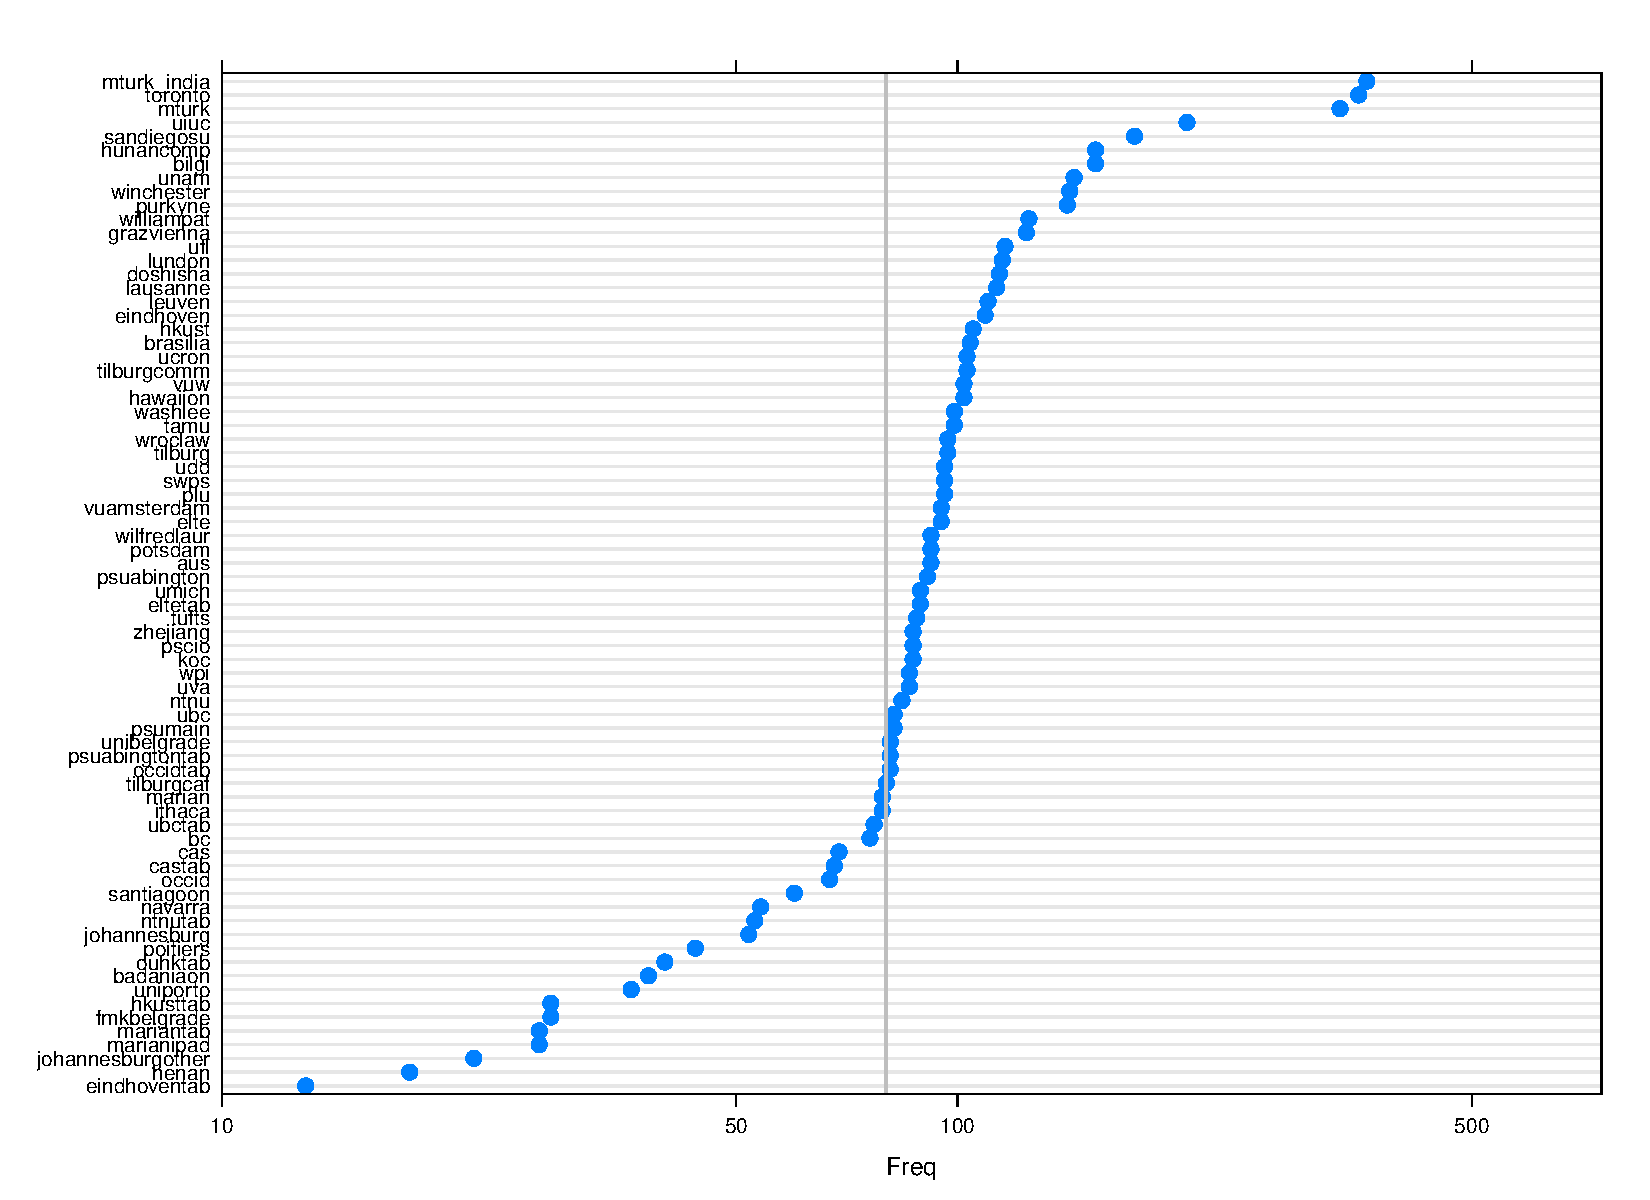
\includegraphics{ML2_data_cleaning_files/figure-latex/unnamed-chunk-33-1.pdf}

\begin{Shaded}
\begin{Highlighting}[]

\NormalTok{S2fr <-}\StringTok{ }\KeywordTok{data.frame}\NormalTok{(}\KeywordTok{ftable}\NormalTok{(ML2.S2$source))}
\NormalTok{S2fr <-}\StringTok{ }\NormalTok{S2fr[}\KeywordTok{order}\NormalTok{(S2fr$Freq), ]}
\KeywordTok{dotplot}\NormalTok{(}\KeywordTok{reorder}\NormalTok{(S2fr$Var1,S2fr$Freq) ~}\StringTok{ }\NormalTok{Freq, }
        \DataTypeTok{scales =} \KeywordTok{list}\NormalTok{(}\DataTypeTok{x =} \KeywordTok{list}\NormalTok{(}\DataTypeTok{log =} \DecValTok{10}\NormalTok{,}\DataTypeTok{at =} \KeywordTok{c}\NormalTok{(}\DecValTok{10}\NormalTok{,}\DecValTok{50}\NormalTok{,}\DecValTok{100}\NormalTok{,}\DecValTok{500}\NormalTok{), }\DataTypeTok{limits =} \KeywordTok{c}\NormalTok{(}\DecValTok{10}\NormalTok{,}\DecValTok{750}\NormalTok{))), }
        \DataTypeTok{data =} \NormalTok{S2fr,}
        \DataTypeTok{panel =} \NormalTok{function (x, y) \{}
                  \KeywordTok{panel.dotplot}\NormalTok{(x,y, }\DataTypeTok{cex=}\FloatTok{1.3}\NormalTok{, }\DataTypeTok{lwd=}\FloatTok{1.5}\NormalTok{)}
                  \KeywordTok{panel.abline}\NormalTok{(}\DataTypeTok{v =} \KeywordTok{log10}\NormalTok{(}\DecValTok{80}\NormalTok{), }\DataTypeTok{col =} \StringTok{"gray"}\NormalTok{, }\DataTypeTok{lwd =} \DecValTok{2}\NormalTok{)}
                  \NormalTok{\}}
        \NormalTok{)}
\end{Highlighting}
\end{Shaded}

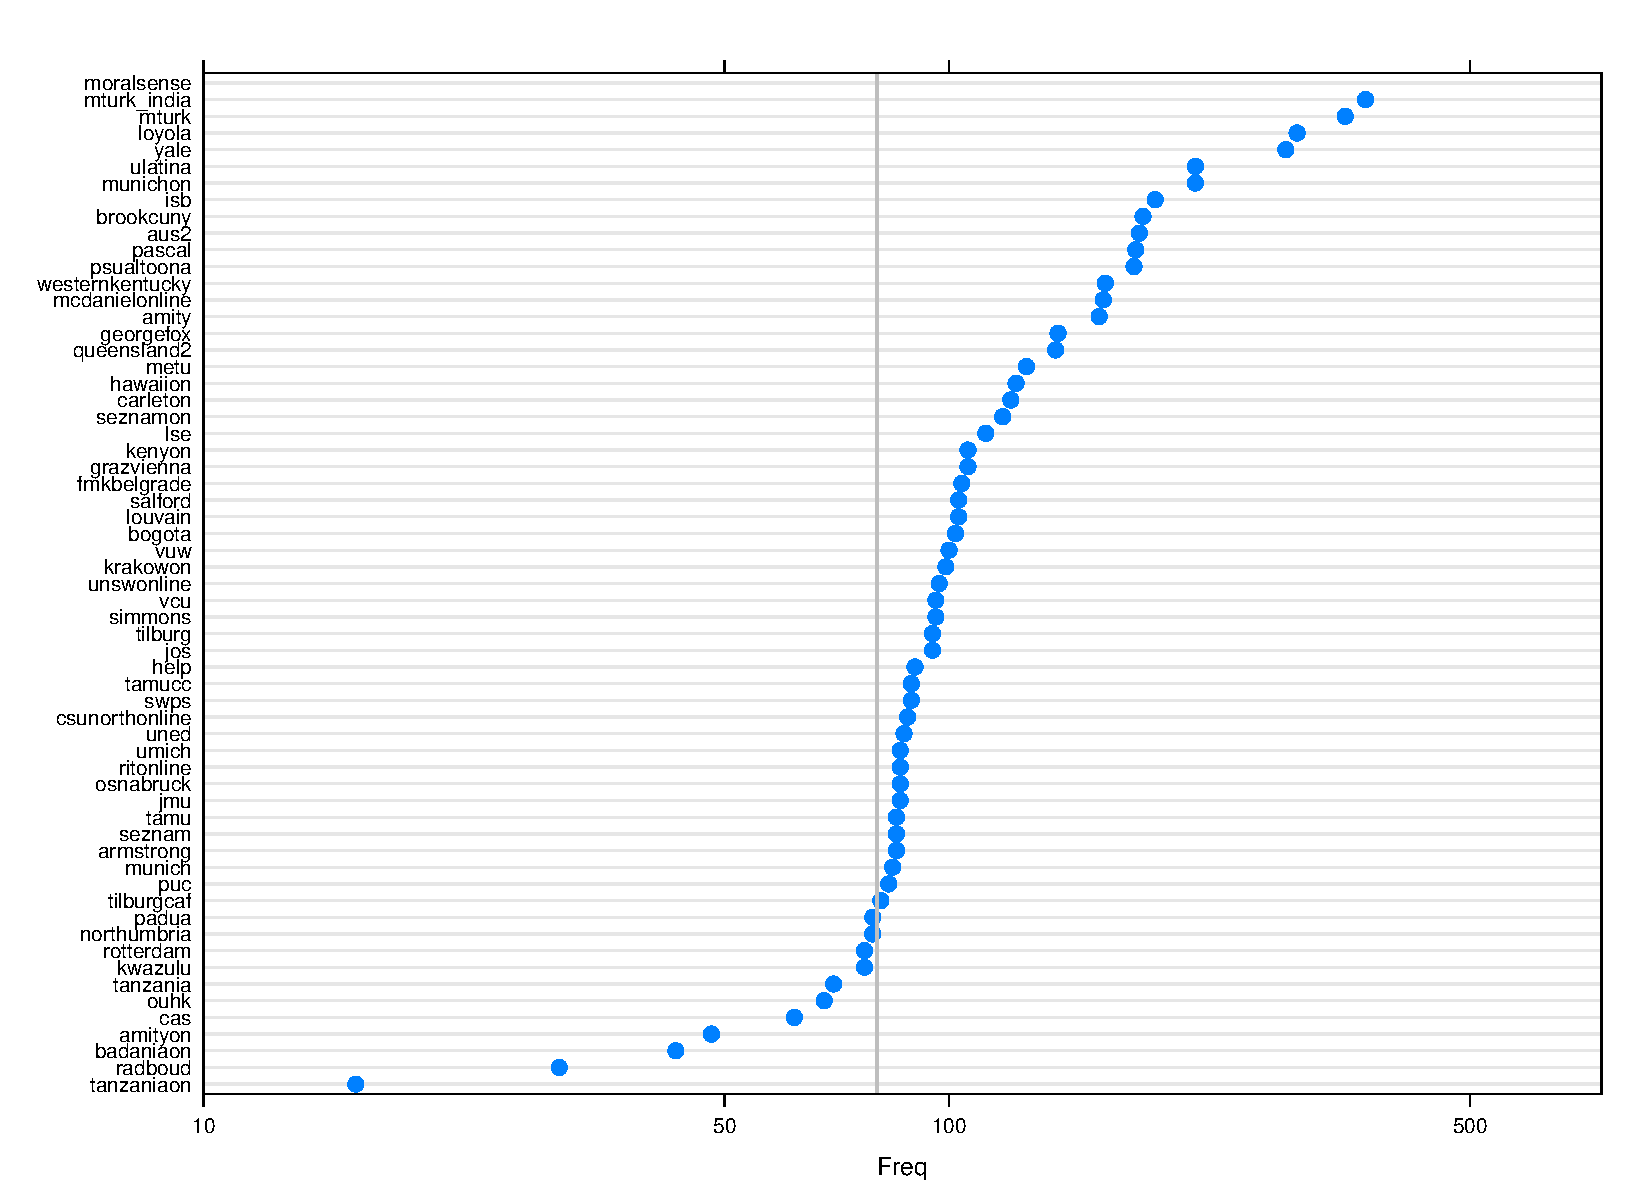
\includegraphics{ML2_data_cleaning_files/figure-latex/unnamed-chunk-33-2.pdf}

\end{document}
